\documentclass[11pt]{article}
\usepackage[margin=0.75in]{geometry}
\usepackage{fontspec}
\IfFontExistsTF{Arial}{\setmainfont{Arial}}{\setmainfont{Latin Modern Roman}}
\usepackage{microtype}
\usepackage{xcolor}
\usepackage{graphicx}
\usepackage{booktabs}
\usepackage{longtable}
\usepackage{array}
\usepackage{tabularx}
\usepackage{float}
\usepackage{enumitem}
\usepackage{hyperref}
\usepackage{xurl}
\usepackage{fancyhdr}
\usepackage{titlesec}
\usepackage{caption}
\usepackage{amsmath}
\hypersetup{colorlinks=true, linkcolor=blue!45!black, urlcolor=blue!45!black, citecolor=blue!45!black}
\definecolor{codexblue}{HTML}{17324D}
\definecolor{codexgold}{HTML}{B9861E}
\definecolor{lightgray}{HTML}{F2F4F8}
\pagestyle{fancy}
\fancyhf{}
\lhead{2026 NBA Draft Big Board}
\rhead{Codex Research Department}
\cfoot{\thepage}
\titleformat{\section}{\Large\bfseries\color{codexblue}}{\thesection}{0.7em}{}
\titleformat{\subsection}{\large\bfseries\color{codexblue}}{\thesubsection}{0.7em}{}
\setlist[itemize]{itemsep=2pt, topsep=3pt}
\setlength{\LTpre}{4pt}
\setlength{\LTpost}{8pt}
\setlength{\tabcolsep}{3pt}
\renewcommand{\arraystretch}{1.08}
\setlength{\parindent}{0pt}
\setlength{\parskip}{6pt}
\emergencystretch=3em
\sloppy
\begin{document}
\begin{titlepage}
\centering
\vspace*{0.6in}
{\Huge\bfseries 2026 NBA Draft Big Board\par}
\vspace{0.18in}
{\Large A LaTeX Research Report from the Codex Scouting Department\par}
\vspace{0.18in}
{\large Current as of 2026-06-10 IST\par}
\vspace{0.5in}
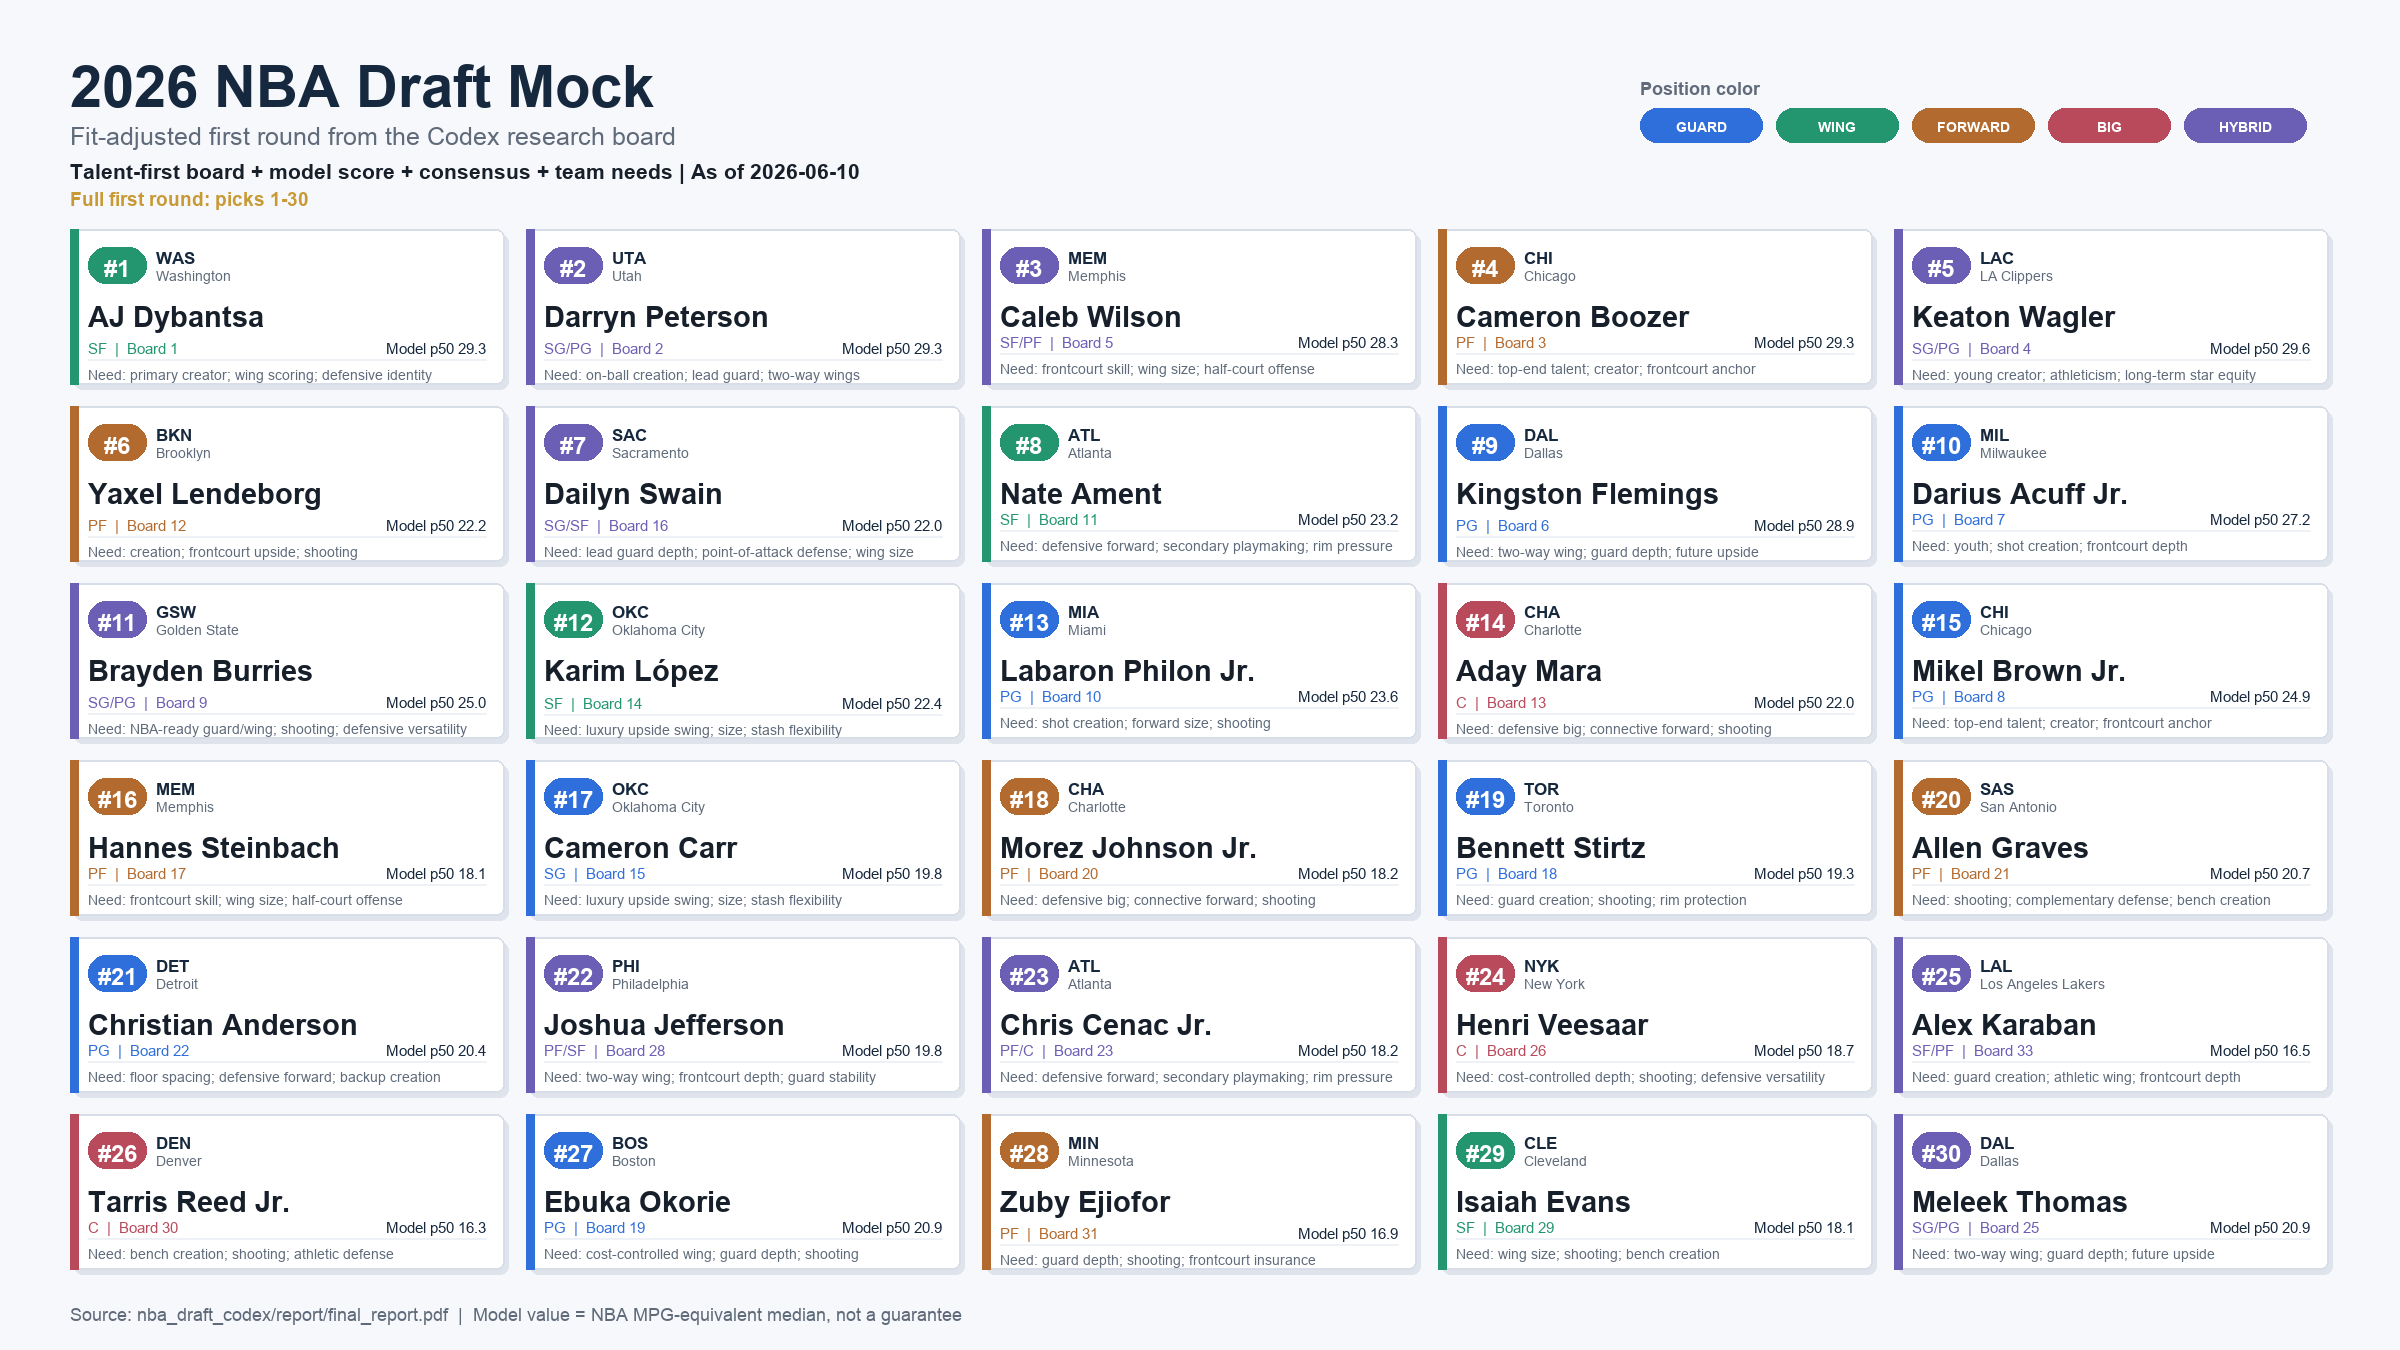
\includegraphics[width=0.94\linewidth]{../figures/shareable_mock_draft_16x9.png}
\vfill
{\large Data, modeling, film-frame protocol, historical comps, and fit-adjusted mock draft\par}
\end{titlepage}
\tableofcontents
\newpage


\section{Abstract}

This report constructs a first-round 2026 NBA Draft big board from live public data collected on 2026-06-10. The final board is led by AJ Dybantsa, Darryn Peterson, Cameron Boozer. The project combines official first-round pick ownership, nine public ranking/mock signals, 2026 combine measurements where recoverable, season production, sourced scouting notes, still-frame film study, a historical draft dataset covering 2000-2021, leave-one-draft-class-out machine learning, bootstrapped uncertainty bands, nearest-neighbor historical comparisons, and team-fit context. The key modeling result is sober rather than flashy: market rank remains the strongest single predictor, and trait models improve the baseline only modestly. Therefore the final board uses a conservative blend of consensus rank, model median value, uncertainty, comps, and film/scouting context.

\section{Introduction and Problem Statement}

The assignment is not merely to list the first thirty prospects. The hard problem is evidence integration: a draft board should separate fetched facts from model inference, and it should distinguish a talent-first ranking from a fit-adjusted mock draft. The output therefore has two ranked artifacts. The big board ranks prospects by expected NBA value. The mock draft maps those prospects onto the actual first-round pick owners and broad roster needs.

This report is written like a Kaggle solution because the model is only useful if it is reproducible and benchmarked. It is written like an academic paper because the validity threats matter as much as the result. The 2026 class includes NCAA freshmen, older college producers, international prospects, and players with uneven samples. That mixture creates missing-data problems and translation-risk problems that should be visible to the reader.

\section{Related Work and Prior Assumptions}

Public draft models have repeatedly found that the market is difficult to beat. Draft slot and consensus rank capture a large amount of dispersed information: live scouting, medical intel, workouts, team interviews, and private measurements. Trait models can still help, especially when they identify statistical profiles that the market underprices, but a model that ignores consensus is likely to overfit. This project therefore treats market rank as the baseline to beat and as an input feature, not as an enemy.

The historical sources include public GitHub draft-model datasets, FiveThirtyEight historical projection data, draft-history/value tables, and combine measurement collections. These sources are imperfect but provide enough scale for a leave-one-draft-class-out validation design. The board also uses public scouting boards from Tankathon, Rookie Scale, CBS, Bleacher Report, Yahoo/KOC, The Ringer, and NBA Draft Room when the HTML snapshot exposed usable data.

\section{Data Collection and Cleaning}

All fetched live data and raw snapshots are logged under data/raw and sources.md. Processed tables live under data/processed. The draft order comes from NBA.com and is used only for the fit-adjusted mock draft; it does not change the pure big board. Prospect statistics primarily come from Tankathon and CBS snapshots. Combine measurements use the NBADraft.net Wayback snapshots plus NBA.com, On3, Yahoo, and NBA Draft Room context where accessible. Several official NBA stats endpoints timed out and Basketball Reference bulk pages returned access blocks; those failures are carried into the limitations rather than hidden.

\begin{center}
\small
\begin{longtable}{@{}>{\raggedright\arraybackslash}p{0.550\linewidth}>{\raggedright\arraybackslash}p{0.220\linewidth}@{}}
\toprule
Source family & Logged entries \\
\midrule
\endfirsthead
\toprule
Source family & Logged entries \\
\midrule
\endhead
Official draft order & 1 \\
Current public boards/mocks & 14 \\
Combine and measurements & 17 \\
Historical modeling data & 27 \\
Film clips and frame archive & 22 \\
Failed/limited endpoints & 7 \\
\bottomrule
\end{longtable}
\end{center}


\subsection{Historical Dataset}

The historical table contains 984 player-seasons/records from draft classes 2000 through 2021, including 520 first-round rows. Rows from 2000-2008 primarily come from the woodfin8 Draft Machine merged data. Rows from 2009-2021 use the JasonG NBA Draft Model data because it has richer pre-draft features and an NBA MPG proxy outcome. Career win shares and VORP are retained where present, but coverage is incomplete enough that the primary supervised target is NBA MPG-equivalent value.

\begin{center}
\small
\begin{longtable}{@{}>{\raggedright\arraybackslash}p{0.550\linewidth}>{\raggedright\arraybackslash}p{0.250\linewidth}@{}}
\toprule
Historical field & Non-null coverage \\
\midrule
\endfirsthead
\toprule
Historical field & Non-null coverage \\
\midrule
\endhead
age\_at\_draft & 62.1\% \\
height\_in & 100.0\% \\
weight\_lbs & 62.1\% \\
wingspan\_in & 34.1\% \\
standing\_reach\_in & 34.1\% \\
ts\_pct & 100.0\% \\
usg\_pct & 60.9\% \\
bpm & 52.6\% \\
outcome\_mpg & 100.0\% \\
career\_vorp & 82.3\% \\
career\_ws & 82.3\% \\
\bottomrule
\end{longtable}
\end{center}


\subsection{Feature Families}

The modeling matrix is intentionally broad but not exotic. Numeric features are: market\_rank, age\_at\_draft, height\_in, weight\_lbs, wingspan\_in, standing\_reach\_in, pts\_per40, reb\_per40, ast\_per40, stl\_per40, blk\_per40, tov\_per40, ts\_pct, usg\_pct, obpm, dbpm, bpm, ft\_pct, three\_pct, three\_pa\_per40. The categorical feature is position\_group. For the comps engine, I used a narrower standardized vector: age\_at\_draft, height\_in, weight\_lbs, wingspan\_in, pts\_per40, reb\_per40, ast\_per40, stl\_per40, blk\_per40, ts\_pct, usg\_pct, bpm. Missing numeric values are median-imputed inside each training fold, and position\_group is most-frequent imputed then one-hot encoded. This matters because several 2026 prospects have incomplete official combine or shooting fields.

\subsection{Outcome Definitions}

The regression target is outcome\_value, defined as NBA MPG-equivalent value in the merged historical dataset. The tier classifier uses five ordered labels: bust, bench, rotation, starter, and star. The tier labels are not the ranking engine; they are probability-flavored context used to communicate floor and ceiling. The report does not claim that an MPG-equivalent model can fully summarize impact, defense, or playoff scalability.

\section{Methodology}

\subsection{Consensus Aggregation}

Player names are normalized across public boards. For every prospect, the pipeline computes source count, mean rank, median rank, minimum rank, maximum rank, and rank standard deviation. The standard deviation is treated as a risk signal: disagreement can indicate role uncertainty, medical uncertainty, sample-size uncertainty, or genuine upside/downside disagreement.

\subsection{Machine Learning Models}

The validation design is leave-one-draft-class-out. For each held-out draft year, every model is trained on all other years and evaluated on the held-out class. This avoids random-row leakage across eras and draft cohorts. The baseline is a ridge regression using only market\_rank. The richer ridge model adds age, measurements, box-score rates, efficiency, usage, BPM components, shooting proxies, and position group. Nonlinear models are gradient boosting regression and random forest regression. A separate gradient boosting classifier predicts outcome tiers.

The specific model family choices are modest by design. Ridge provides interpretability and a strong regularized baseline. Gradient boosting captures nonlinear interactions such as age-by-production or size-by-role without requiring deep learning scale. Random forest is used as a robustness check. The bootstrap uncertainty band samples historical draft years with replacement and fits eighty shallow gradient boosting models; the reported p10/p50/p90 for 2026 prospects are percentiles of those bootstrap predictions.

\subsection{Final Board Formula}

Because the learned models only modestly beat the market baseline, the final board is a blended ranking rather than a pure model sort. The board score is:

\[ S = 0.68(-z_{\mathrm{consensus}}) + 0.27 z_{\mathrm{model}} - 0.05 z_{\mathrm{spread}} \]

where lower consensus rank is better, model is predicted p50 MPG-equivalent value, and spread is public-rank standard deviation. This weighting anchors the board to the strongest signal while still allowing model value and disagreement risk to move prospects within tiers.

\subsection{Historical Comps Engine}

The comps engine standardizes age, height, weight, wingspan, per-40 production, efficiency, usage, and BPM, then fits a five-nearest-neighbor model with Euclidean distance. Every comp cohort is empirical: the low, median, and high outcomes are the actual NBA MPG-equivalent outcomes of those historical neighbors. A comp is not claimed as a stylistic clone. It is a statistical-profile neighbor, and the report flags this distinction throughout.

\section{Model Results}

\begin{center}
\small
\begin{longtable}{@{}>{\raggedright\arraybackslash}p{0.460\linewidth}>{\raggedright\arraybackslash}p{0.140\linewidth}>{\raggedright\arraybackslash}p{0.140\linewidth}>{\raggedright\arraybackslash}p{0.160\linewidth}@{}}
\toprule
Model & MAE & RMSE & Spearman \\
\midrule
\endfirsthead
\toprule
Model & MAE & RMSE & Spearman \\
\midrule
\endhead
Ridge baseline, market rank only & 6.059 & 7.288 & 0.634 \\
Ridge, market plus traits & 5.966 & 7.220 & 0.644 \\
Gradient boosting, market plus traits & 5.963 & 7.329 & 0.621 \\
Random forest, market plus traits & 5.895 & 7.266 & 0.630 \\
\bottomrule
\end{longtable}
\end{center}


The market-only baseline posted MAE 6.059, RMSE 7.288, and Spearman 0.634. The random forest posted the best MAE at 5.895; ridge with traits posted the best rank correlation at 0.644. This is a narrow win, not a model landslide. The main conclusion is that model output is useful as a board modifier, but the public market remains the dominant prior.

\subsection{Classifier}

The tier classifier accuracy is 0.394. Its confusion matrix shows the expected draft-model problem: stars and busts are hard to separate from adjacent outcomes, and many true starters/rotation players collapse into the middle classes.

\begin{center}
\scriptsize
\begin{longtable}{@{}>{\raggedright\arraybackslash}p{0.160\linewidth}>{\raggedright\arraybackslash}p{0.140\linewidth}>{\raggedright\arraybackslash}p{0.140\linewidth}>{\raggedright\arraybackslash}p{0.140\linewidth}>{\raggedright\arraybackslash}p{0.140\linewidth}>{\raggedright\arraybackslash}p{0.140\linewidth}@{}}
\toprule
Actual & bust & bench & rotation & starter & star \\
\midrule
\endfirsthead
\toprule
Actual & bust & bench & rotation & starter & star \\
\midrule
\endhead
bust & 92 & 41 & 43 & 1 & 3 \\
bench & 57 & 61 & 107 & 13 & 0 \\
rotation & 24 & 62 & 190 & 34 & 5 \\
starter & 4 & 24 & 101 & 36 & 19 \\
star & 2 & 2 & 23 & 31 & 9 \\
\bottomrule
\end{longtable}
\end{center}


\subsection{Feature Importance}

Permutation importance confirms the central lesson. Market rank dominates. Secondary signals with meaningful but much smaller importance include assist production, age, turnovers, block/steal production, scoring volume, and shooting indicators. This aligns with the final-board design: a smart board can move from consensus, but it should not pretend that a small public feature set fully replaces the market.

\begin{center}
\small
\begin{longtable}{@{}>{\raggedright\arraybackslash}p{0.460\linewidth}>{\raggedright\arraybackslash}p{0.320\linewidth}@{}}
\toprule
Feature & Permutation MAE increase \\
\midrule
\endfirsthead
\toprule
Feature & Permutation MAE increase \\
\midrule
\endhead
market\_rank & 3.334 \\
ast\_per40 & 0.214 \\
age\_at\_draft & 0.093 \\
tov\_per40 & 0.089 \\
blk\_per40 & 0.089 \\
pts\_per40 & 0.083 \\
three\_pct & 0.079 \\
stl\_per40 & 0.078 \\
bpm & 0.071 \\
reb\_per40 & 0.061 \\
dbpm & 0.051 \\
height\_in & 0.046 \\
three\_pa\_per40 & 0.046 \\
obpm & 0.040 \\
ft\_pct & 0.028 \\
\bottomrule
\end{longtable}
\end{center}


\begin{figure}[H]\centering
\includegraphics[width=0.92\linewidth]{../figures/feature_importance.png}\caption{Permutation importance for the final gradient boosting model.}\end{figure}

\begin{figure}[H]\centering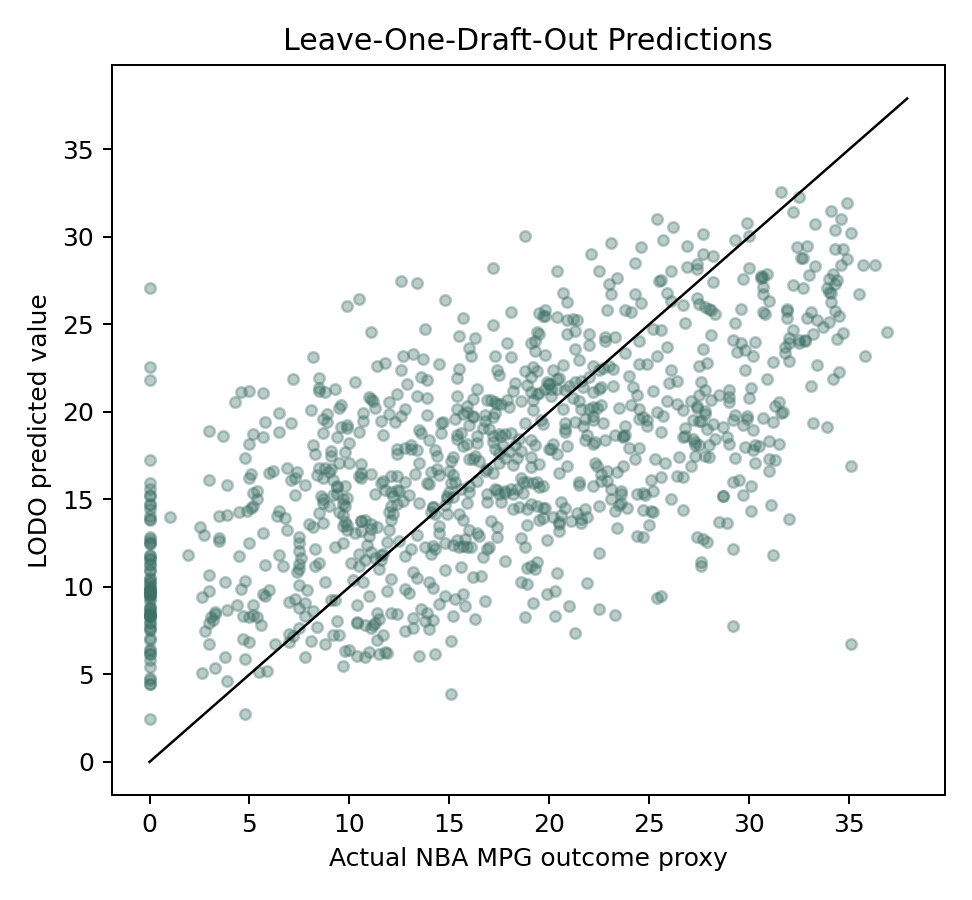
\includegraphics[width=0.82\linewidth]{../figures/cv_predicted_vs_actual.png}\caption{Leave-one-draft-class-out predictions versus actual NBA MPG-equivalent outcome.}\end{figure}

\section{Board-Level Figures}

\begin{figure}[H]\centering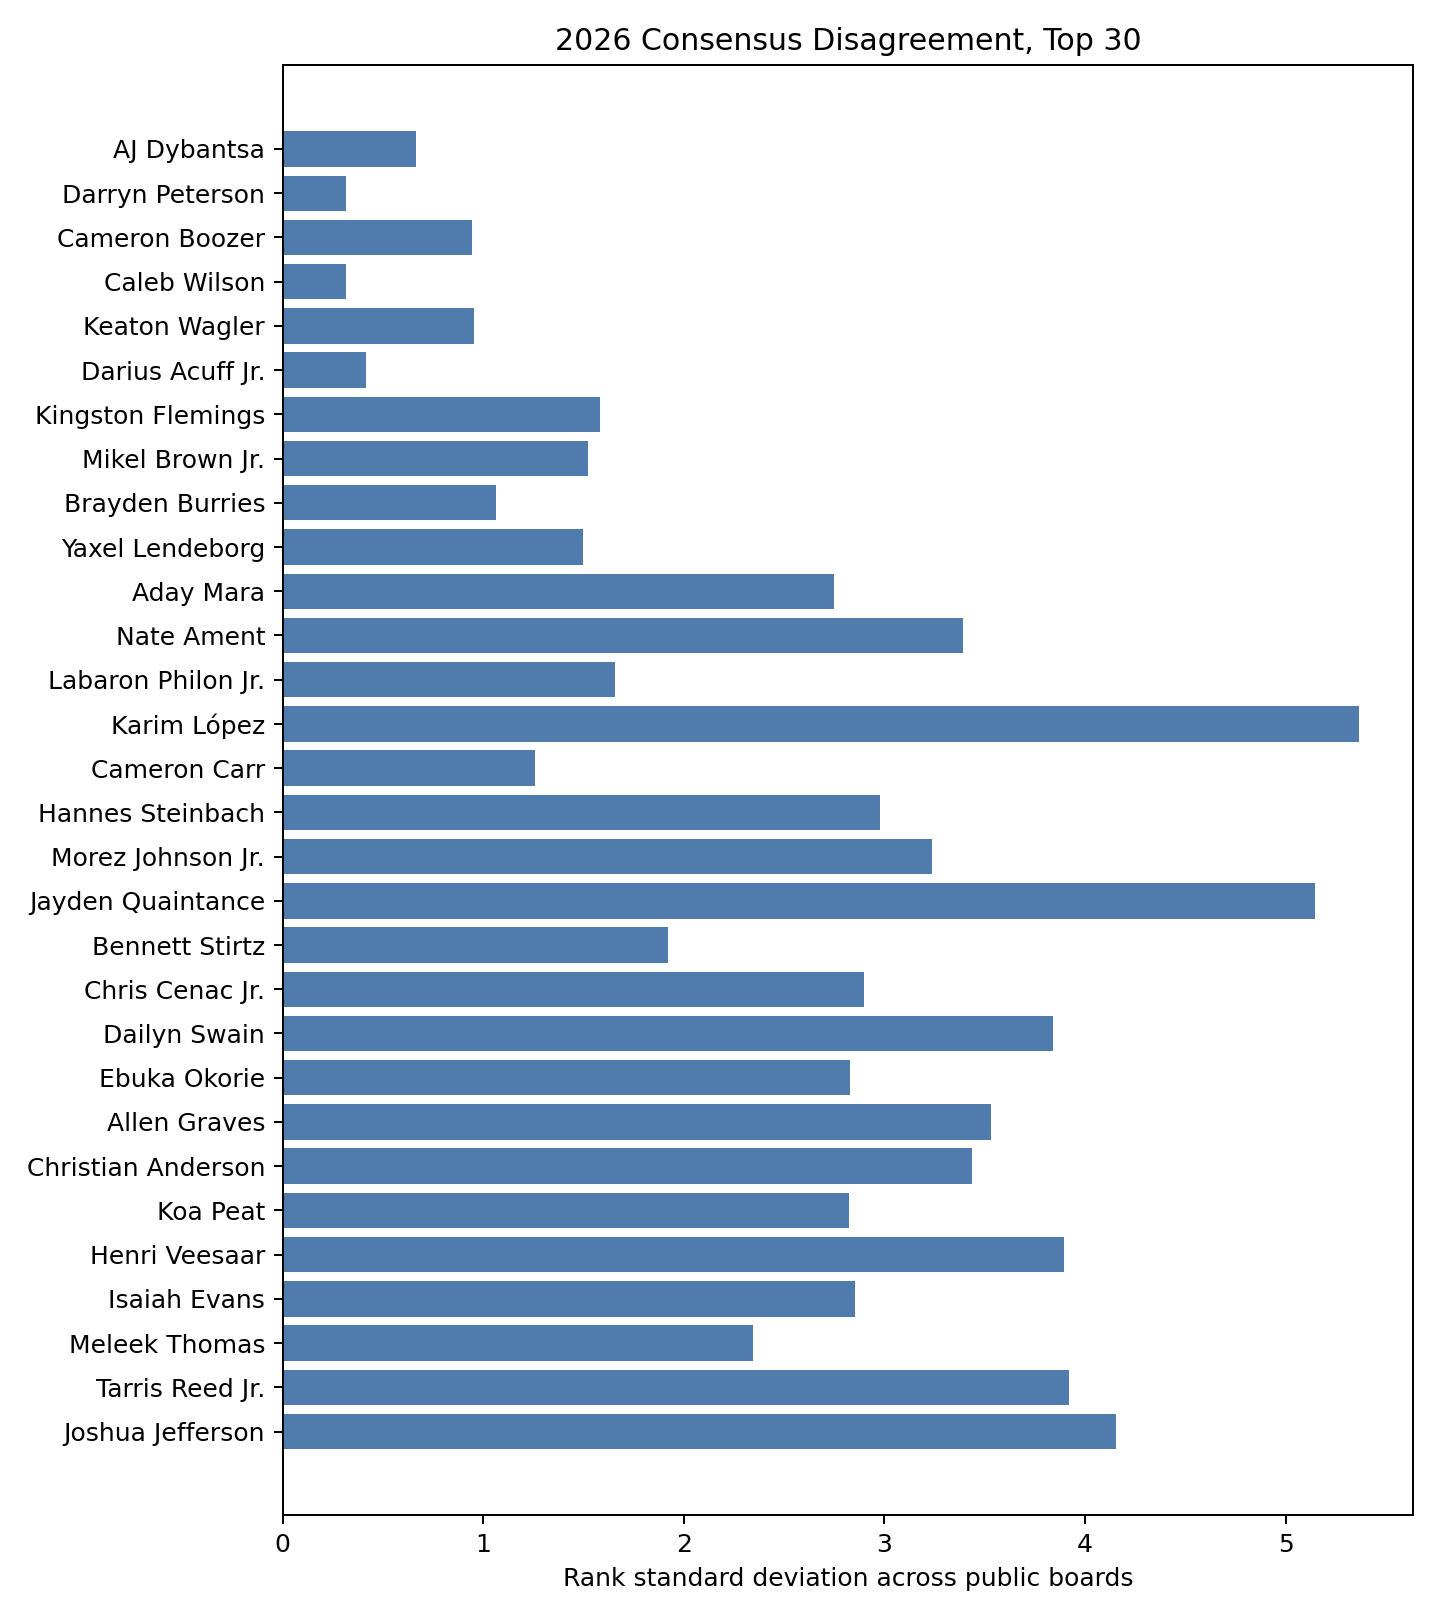
\includegraphics[width=0.95\linewidth]{../figures/consensus_spread_top30.png}\caption{Public-board disagreement among top prospects. Spread is used as a risk feature.}\end{figure}

\begin{figure}[H]\centering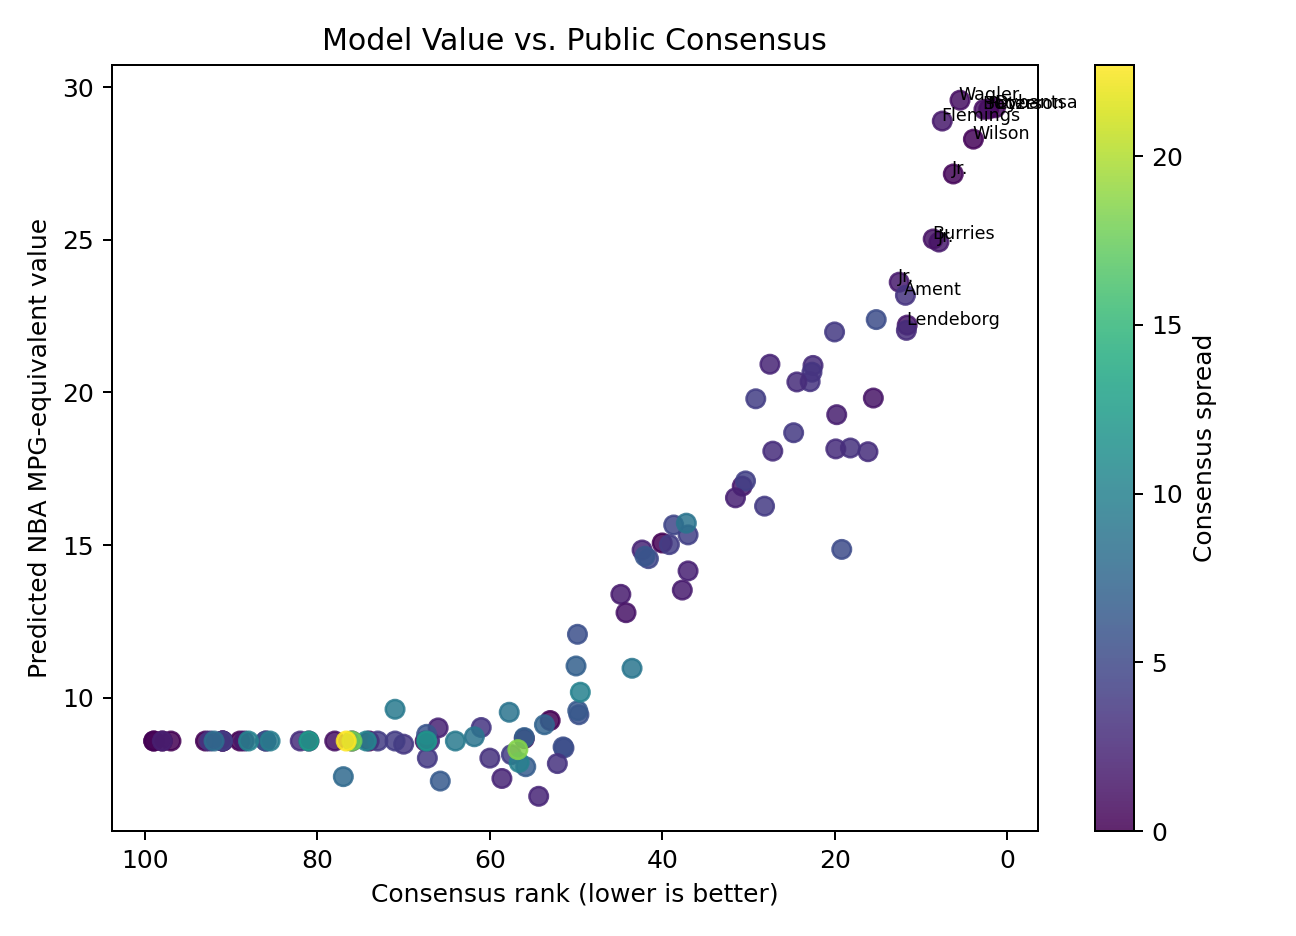
\includegraphics[width=0.88\linewidth]{../figures/model_vs_consensus.png}\caption{Model value versus consensus rank; color encodes consensus spread.}\end{figure}

\begin{figure}[H]\centering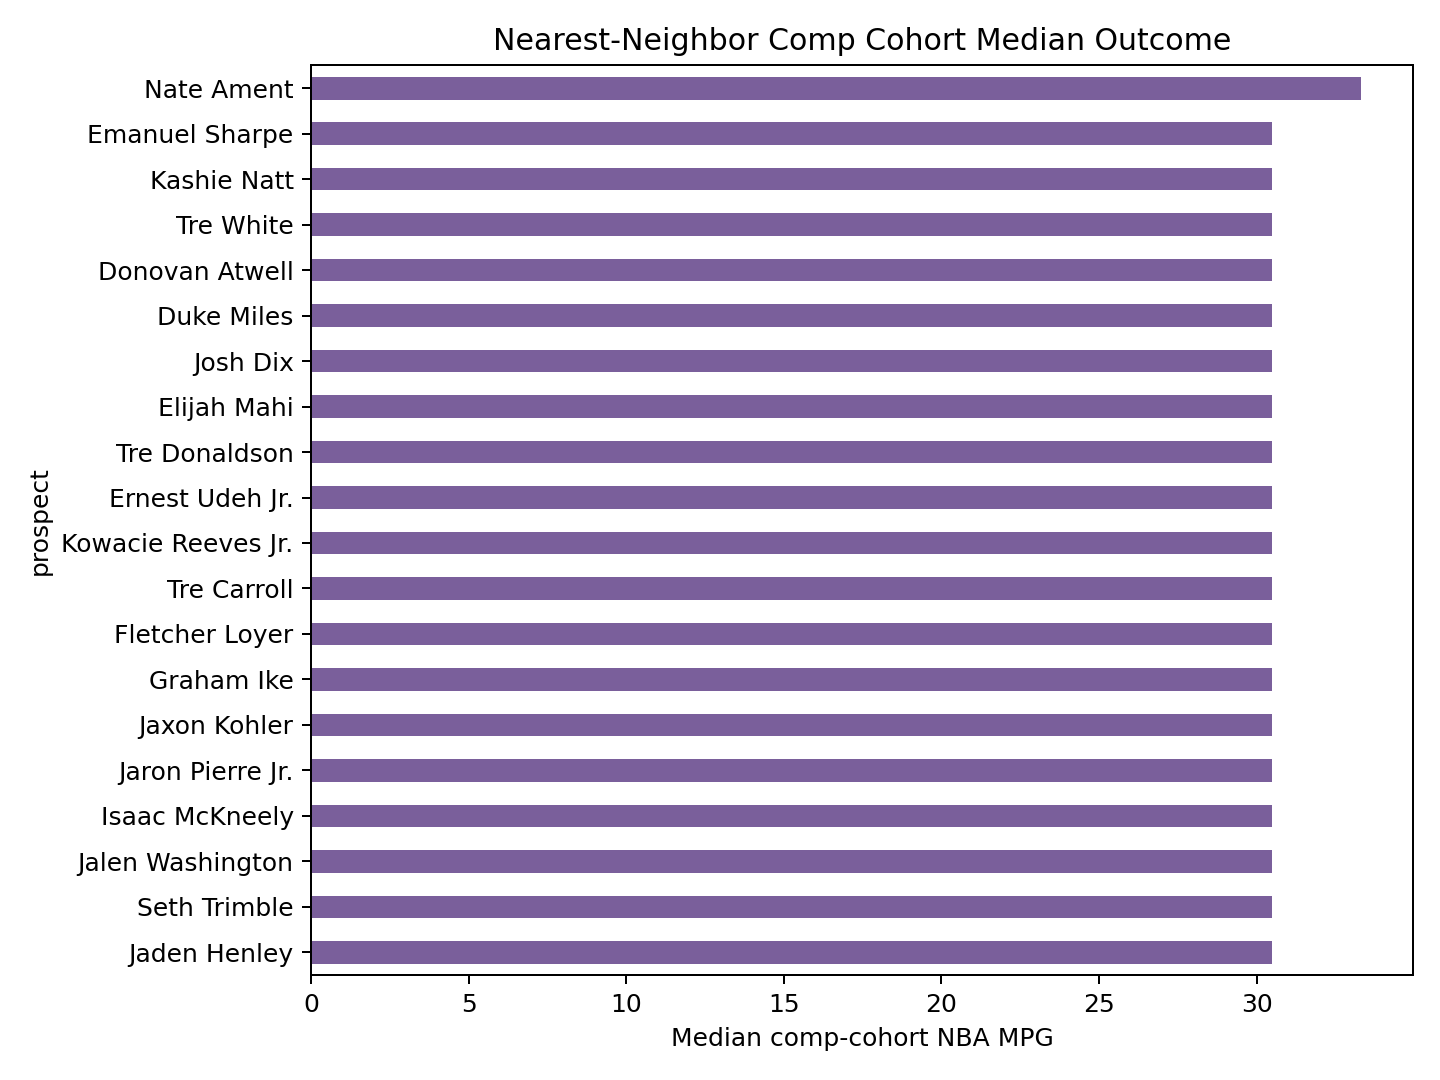
\includegraphics[width=0.92\linewidth]{../figures/comp_cohort_medians.png}\caption{Median NBA MPG outcome of nearest-neighbor historical comp cohorts.}\end{figure}

\section{Film Study: Protocol and Representative Frames}
The film component is intentionally conservative. Public clips were downloaded or imported through a local yt-dlp/ffmpeg archive, frames were sampled, and notes were written with two separate buckets: frame-based observations made from still images, and sourced human scouting observations. A still frame can support a claim about body position, release point, gather height, handle posture, or the presence of a contest. It cannot support a confident claim about burst, processing speed, screen navigation timing, defensive reaction time, or live advantage creation. Those claims remain sourced human-scouting context, not model evidence.

For the top ten, I selected up to four illustrative frames per prospect. They are included below as evidence examples, not as a substitute for full-game film charting.
\subsection{AJ Dybantsa: selected still frames}
\begin{figure}[H]\centering

\includegraphics[width=0.48\linewidth]{../film/frames/_report_picks/dybantsa_pick1.jpg}

\includegraphics[width=0.48\linewidth]{../film/frames/_report_picks/dybantsa_pick2.jpg}

\includegraphics[width=0.48\linewidth]{../film/frames/_report_picks/dybantsa_pick3.jpg}

\includegraphics[width=0.48\linewidth]{../film/frames/_report_picks/dybantsa_pick4.jpg}
\caption{Selected frame samples for AJ Dybantsa. These images support only the static observations discussed in the notes.}
\end{figure}
\subsection{Darryn Peterson: selected still frames}
\begin{figure}[H]\centering

\includegraphics[width=0.48\linewidth]{../film/frames/_report_picks/peterson_pick1.jpg}

\includegraphics[width=0.48\linewidth]{../film/frames/_report_picks/peterson_pick2.jpg}

\includegraphics[width=0.48\linewidth]{../film/frames/_report_picks/peterson_pick3.jpg}

\includegraphics[width=0.48\linewidth]{../film/frames/_report_picks/peterson_pick4.jpg}
\caption{Selected frame samples for Darryn Peterson. These images support only the static observations discussed in the notes.}
\end{figure}
\subsection{Cameron Boozer: selected still frames}
\begin{figure}[H]\centering

\includegraphics[width=0.48\linewidth]{../film/frames/_report_picks/boozer_pick1.jpg}

\includegraphics[width=0.48\linewidth]{../film/frames/_report_picks/boozer_pick2.jpg}

\includegraphics[width=0.48\linewidth]{../film/frames/_report_picks/boozer_pick3.jpg}

\includegraphics[width=0.48\linewidth]{../film/frames/_report_picks/boozer_pick4.jpg}
\caption{Selected frame samples for Cameron Boozer. These images support only the static observations discussed in the notes.}
\end{figure}
\subsection{Keaton Wagler: selected still frames}
\begin{figure}[H]\centering

\includegraphics[width=0.48\linewidth]{../film/frames/_report_picks/wagler_pick1.jpg}

\includegraphics[width=0.48\linewidth]{../film/frames/_report_picks/wagler_pick2.jpg}

\includegraphics[width=0.48\linewidth]{../film/frames/_report_picks/wagler_pick3.jpg}

\includegraphics[width=0.48\linewidth]{../film/frames/_report_picks/wagler_pick4.jpg}
\caption{Selected frame samples for Keaton Wagler. These images support only the static observations discussed in the notes.}
\end{figure}
\subsection{Caleb Wilson: selected still frames}
\begin{figure}[H]\centering

\includegraphics[width=0.48\linewidth]{../film/frames/_report_picks/wilson_pick1.jpg}

\includegraphics[width=0.48\linewidth]{../film/frames/_report_picks/wilson_pick2.jpg}

\includegraphics[width=0.48\linewidth]{../film/frames/_report_picks/wilson_pick3.jpg}

\includegraphics[width=0.48\linewidth]{../film/frames/_report_picks/wilson_pick4.jpg}
\caption{Selected frame samples for Caleb Wilson. These images support only the static observations discussed in the notes.}
\end{figure}
\subsection{Kingston Flemings: selected still frames}
\begin{figure}[H]\centering

\includegraphics[width=0.48\linewidth]{../film/frames/_report_picks/flemings_pick1.jpg}

\includegraphics[width=0.48\linewidth]{../film/frames/_report_picks/flemings_pick2.jpg}

\includegraphics[width=0.48\linewidth]{../film/frames/_report_picks/flemings_pick3.jpg}

\includegraphics[width=0.48\linewidth]{../film/frames/_report_picks/flemings_pick4.jpg}
\caption{Selected frame samples for Kingston Flemings. These images support only the static observations discussed in the notes.}
\end{figure}
\subsection{Darius Acuff Jr.: selected still frames}
\begin{figure}[H]\centering

\includegraphics[width=0.48\linewidth]{../film/frames/_report_picks/acuff_pick1.jpg}

\includegraphics[width=0.48\linewidth]{../film/frames/_report_picks/acuff_pick2.jpg}

\includegraphics[width=0.48\linewidth]{../film/frames/_report_picks/acuff_pick3.jpg}

\includegraphics[width=0.48\linewidth]{../film/frames/_report_picks/acuff_pick4.jpg}
\caption{Selected frame samples for Darius Acuff Jr.. These images support only the static observations discussed in the notes.}
\end{figure}
\subsection{Mikel Brown Jr.: selected still frames}
\begin{figure}[H]\centering

\includegraphics[width=0.48\linewidth]{../film/frames/_report_picks/brown_mikel_pick1.jpg}

\includegraphics[width=0.48\linewidth]{../film/frames/_report_picks/brown_mikel_pick2.jpg}

\includegraphics[width=0.48\linewidth]{../film/frames/_report_picks/brown_mikel_pick3.jpg}
\caption{Selected frame samples for Mikel Brown Jr.. These images support only the static observations discussed in the notes.}
\end{figure}
\subsection{Brayden Burries: selected still frames}
\begin{figure}[H]\centering

\includegraphics[width=0.48\linewidth]{../film/frames/_report_picks/burries_pick1.jpg}

\includegraphics[width=0.48\linewidth]{../film/frames/_report_picks/burries_pick2.jpg}

\includegraphics[width=0.48\linewidth]{../film/frames/_report_picks/burries_pick3.jpg}

\includegraphics[width=0.48\linewidth]{../film/frames/_report_picks/burries_pick4.jpg}
\caption{Selected frame samples for Brayden Burries. These images support only the static observations discussed in the notes.}
\end{figure}
\subsection{Labaron Philon Jr.: selected still frames}
\begin{figure}[H]\centering
\includegraphics[width=0.48\linewidth]{../film/frames/_report_picks/philon_pick1.jpg}
\includegraphics[width=0.48\linewidth]{../film/frames/_report_picks/philon_pick2.jpg}
\includegraphics[width=0.48\linewidth]{../film/frames/_report_picks/philon_pick3.jpg}
\includegraphics[width=0.48\linewidth]{../film/frames/_report_picks/philon_pick4.jpg}
\caption{Selected frame samples for Labaron Philon Jr.. These images support only the static observations discussed in the notes.}
\end{figure}


\section{The 2026 Talent-First Big Board}

The table below is the pure board. It is not a mock draft. The model value is an NBA MPG-equivalent median with a bootstrapped p10-p90 band, not a guaranteed minute projection.

\begin{center}
\scriptsize
\begin{longtable}{@{}>{\raggedright\arraybackslash}p{0.055\linewidth}>{\raggedright\arraybackslash}p{0.164\linewidth}>{\raggedright\arraybackslash}p{0.073\linewidth}>{\raggedright\arraybackslash}p{0.146\linewidth}>{\raggedright\arraybackslash}p{0.064\linewidth}>{\raggedright\arraybackslash}p{0.091\linewidth}>{\raggedright\arraybackslash}p{0.155\linewidth}>{\raggedright\arraybackslash}p{0.173\linewidth}@{}}
\toprule
Rank & Prospect & Pos & Team/School & Age & Consensus & Model p50 [p10,p90] & Tier \\
\midrule
\endfirsthead
\toprule
Rank & Prospect & Pos & Team/School & Age & Consensus & Model p50 [p10,p90] & Tier \\
\midrule
\endhead
1 & AJ Dybantsa & SF & BYU & 19.4 & 1.3 & 29.3 [28.0, 31.4] & Tier 1: primary star bets \\
2 & Darryn Peterson & SG/PG & Kansas & 19.4 & 2.1 & 29.3 [27.6, 30.8] & Tier 1: primary star bets \\
3 & Cameron Boozer & PF & Duke & 18.9 & 2.7 & 29.3 [27.3, 30.7] & Tier 1: primary star bets \\
4 & Keaton Wagler & SG/PG & Illinois & 19.4 & 5.4 & 29.6 [28.5, 30.8] & Tier 2: high-lottery starters \\
5 & Caleb Wilson & SF/PF & North Carolina & 19.9 & 3.9 & 28.3 [26.9, 30.3] & Tier 2: high-lottery starters \\
6 & Kingston Flemings & PG & Houston & 19.5 & 7.5 & 28.9 [26.4, 30.7] & Tier 2: high-lottery starters \\
7 & Darius Acuff Jr. & PG & Arkansas & 19.6 & 6.2 & 27.2 [25.5, 29.1] & Tier 2: high-lottery starters \\
8 & Mikel Brown Jr. & PG & Louisville & 20.2 & 7.9 & 24.9 [23.2, 26.9] & Tier 2: high-lottery starters \\
9 & Brayden Burries & SG/PG & Arizona & 20.8 & 8.6 & 25.0 [23.2, 26.8] & Tier 3: starter/plus-rotation bets \\
10 & Labaron Philon Jr. & PG & Alabama & 20.6 & 12.5 & 23.6 [21.4, 25.1] & Tier 3: starter/plus-rotation bets \\
11 & Nate Ament & SF & Tennessee & 19.5 & 11.8 & 23.2 [21.8, 24.7] & Tier 3: starter/plus-rotation bets \\
12 & Yaxel Lendeborg & PF & Michigan & 23.7 & 11.6 & 22.2 [20.7, 23.5] & Tier 3: starter/plus-rotation bets \\
13 & Aday Mara & C & Michigan & 21.2 & 11.7 & 22.0 [19.5, 25.1] & Tier 3: starter/plus-rotation bets \\
14 & Karim López & SF & New Zealand & 19.2 & 15.2 & 22.4 [20.7, 23.5] & Tier 3: starter/plus-rotation bets \\
15 & Cameron Carr & SG & Baylor & 21.6 & 15.5 & 19.8 [18.4, 21.3] & Tier 4: rotation upside \\
16 & Dailyn Swain & SG/SF & Texas & 20.9 & 20.0 & 22.0 [20.7, 23.4] & Tier 4: rotation upside \\
17 & Hannes Steinbach & PF & Washington & 20.1 & 16.1 & 18.1 [16.5, 20.2] & Tier 4: rotation upside \\
18 & Bennett Stirtz & PG & Iowa & 22.7 & 19.8 & 19.3 [17.9, 20.3] & Tier 4: rotation upside \\
19 & Ebuka Okorie & PG & Stanford & 19.2 & 22.5 & 20.9 [19.2, 22.9] & Tier 4: rotation upside \\
20 & Morez Johnson Jr. & PF & Michigan & 20.4 & 18.2 & 18.2 [16.7, 19.8] & Tier 4: rotation upside \\
21 & Allen Graves & PF & Santa Clara & 19.9 & 22.6 & 20.7 [17.7, 22.9] & Tier 4: rotation upside \\
22 & Christian Anderson & PG & Texas Tech & 20.2 & 22.8 & 20.4 [18.6, 22.0] & Tier 4: rotation upside \\
23 & Chris Cenac Jr. & PF/C & Houston & 19.4 & 19.9 & 18.2 [16.5, 19.7] & Tier 4: rotation upside \\
24 & Koa Peat & PF & Arizona & 19.4 & 24.4 & 20.3 [19.2, 21.4] & Tier 4: rotation upside \\
25 & Meleek Thomas & SG/PG & Arkansas & 19.9 & 27.5 & 20.9 [19.2, 22.5] & Tier 5: first-round value \\
26 & Henri Veesaar & C & North Carolina & 22.2 & 24.8 & 18.7 [17.2, 20.0] & Tier 5: first-round value \\
27 & Jayden Quaintance & PF/C & Kentucky & 18.9 & 19.2 & 14.9 [12.9, 17.5] & Tier 5: first-round value \\
28 & Joshua Jefferson & PF/SF & Iowa State & 22.6 & 29.1 & 19.8 [17.6, 21.3] & Tier 5: first-round value \\
29 & Isaiah Evans & SF & Duke & 20.5 & 27.2 & 18.1 [16.5, 19.1] & Tier 5: first-round value \\
30 & Tarris Reed Jr. & C & UConn & 22.9 & 28.1 & 16.3 [14.5, 18.7] & Tier 5: first-round value \\
\bottomrule
\end{longtable}
\end{center}


\subsection{1. AJ Dybantsa}
\begin{center}
\scriptsize
\begin{longtable}{@{}>{\raggedright\arraybackslash}p{0.230\linewidth}>{\raggedright\arraybackslash}p{0.680\linewidth}@{}}
\toprule
Field & Value \\
\midrule
\endfirsthead
\toprule
Field & Value \\
\midrule
\endhead
Tier & Tier 1: primary star bets \\
Position / school & SF, BYU \\
Age at draft & 19.4 \\
Measurements & 80.5 in, 217.0 lb, 84.5 in wingspan, 106.0 in reach \\
Production & 25.5 PPG, 6.8 RPG, 3.7 APG, 1.1 SPG, 0.3 BPG \\
Efficiency / impact & TS 0.600, usage 33.9, BPM 11.7 \\
Consensus & mean 1.3, median 1.0, spread 0.7, range 1-3 \\
Model value & p10 28.0, p50 29.3, p90 31.4 MPG-equivalent \\
Tier probabilities & bust 2\%, rotation 18\%, starter 37\%, star 40\% \\
\bottomrule
\end{longtable}
\end{center}

\paragraph{Ranking rationale.}
\begin{itemize}[leftmargin=*]
\item Codex rank is close to the public market, so the board treats this as an evidence-aligned slot rather than a strong contrarian call.
\item The model median (29.3 MPG-equivalent) is comfortably above the 2026 prospect-pool median.
\item Age at draft (19.4) is a positive developmental signal in this model family.
\item Wingspan differential is positive at roughly +4.0 inches.
\end{itemize}
\paragraph{Nearest-neighbor comps.}
\begin{center}
\scriptsize
\begin{longtable}{@{}>{\raggedright\arraybackslash}p{0.060\linewidth}>{\raggedright\arraybackslash}p{0.280\linewidth}>{\raggedright\arraybackslash}p{0.100\linewidth}>{\raggedright\arraybackslash}p{0.100\linewidth}>{\raggedright\arraybackslash}p{0.160\linewidth}>{\raggedright\arraybackslash}p{0.160\linewidth}@{}}
\toprule
\# & Historical comp & Year & Pick & Outcome MPG & Tier \\
\midrule
\endfirsthead
\toprule
\# & Historical comp & Year & Pick & Outcome MPG & Tier \\
\midrule
\endhead
1 & RJ Barrett & 2019 & 3 & 33.3 & star \\
2 & TJ Warren & 2014 & 14 & 27.4 & starter \\
3 & Jarrett Culver & 2019 & 6 & 17.2 & rotation \\
4 & Alec Burks & 2011 & 12 & 22.8 & rotation \\
5 & Cade Cunningham & 2021 & 1 & 33.3 & star \\
\bottomrule
\end{longtable}
\end{center}

\paragraph{Frame-based film observations (mine).}
\begin{itemize}[leftmargin=*]
\item Jump shot, elevated release. On a left-wing jumper vs Abilene Christian (frame\_0544.jpg, ball flight in frame\_0547.jpg), the ball leaves above and slightly in front of his head with full arm extension at the top of the jump. The release point sits well above the closest defender's contest. Frames cannot show the rhythm or speed of the load, only that the...
\item Free throw setup, squared and narrow-calm base (frame\_0549.jpg, frame\_0550.jpg, frame\_0551.jpg). Close-ups at the line show shoulders level, eyes fixed on the rim, and a relaxed neutral posture before the dip. The broadcast framing crops the lower body, so base width at the line cannot be fully judged from these frames.
\end{itemize}
\paragraph{Sourced scouting cross-check.}
Human scouting sources consulted in the note file: Babcock Hoops scouting report, Deseret News, HoopsHype. I use these directionally and avoid treating still frames as live-film evidence.


\subsection{2. Darryn Peterson}
\begin{center}
\scriptsize
\begin{longtable}{@{}>{\raggedright\arraybackslash}p{0.230\linewidth}>{\raggedright\arraybackslash}p{0.680\linewidth}@{}}
\toprule
Field & Value \\
\midrule
\endfirsthead
\toprule
Field & Value \\
\midrule
\endhead
Tier & Tier 1: primary star bets \\
Position / school & SG/PG, Kansas \\
Age at draft & 19.4 \\
Measurements & 76.5 in, 198.8 lb, 81.8 in wingspan, 103.0 in reach \\
Production & 20.2 PPG, 4.2 RPG, 1.6 APG, 1.4 SPG, 0.6 BPG \\
Efficiency / impact & TS 0.578, usage 33.5, BPM 14.1 \\
Consensus & mean 2.1, median 2.0, spread 0.3, range 2-3 \\
Model value & p10 27.6, p50 29.3, p90 30.8 MPG-equivalent \\
Tier probabilities & bust 2\%, rotation 19\%, starter 52\%, star 21\% \\
\bottomrule
\end{longtable}
\end{center}

\paragraph{Ranking rationale.}
\begin{itemize}[leftmargin=*]
\item Codex rank is close to the public market, so the board treats this as an evidence-aligned slot rather than a strong contrarian call.
\item The model median (29.3 MPG-equivalent) is comfortably above the 2026 prospect-pool median.
\item Age at draft (19.4) is a positive developmental signal in this model family.
\item Wingspan differential is positive at roughly +5.2 inches.
\end{itemize}
\paragraph{Nearest-neighbor comps.}
\begin{center}
\scriptsize
\begin{longtable}{@{}>{\raggedright\arraybackslash}p{0.060\linewidth}>{\raggedright\arraybackslash}p{0.280\linewidth}>{\raggedright\arraybackslash}p{0.100\linewidth}>{\raggedright\arraybackslash}p{0.100\linewidth}>{\raggedright\arraybackslash}p{0.160\linewidth}>{\raggedright\arraybackslash}p{0.160\linewidth}@{}}
\toprule
\# & Historical comp & Year & Pick & Outcome MPG & Tier \\
\midrule
\endfirsthead
\toprule
\# & Historical comp & Year & Pick & Outcome MPG & Tier \\
\midrule
\endhead
1 & Kentavious Caldwell-Pope & 2013 & 8 & 29.6 & starter \\
2 & Jarrett Culver & 2019 & 6 & 17.2 & rotation \\
3 & DAngelo Russell & 2015 & 2 & 29.9 & starter \\
4 & TJ Warren & 2014 & 14 & 27.4 & starter \\
5 & Klay Thompson & 2011 & 11 & 32.8 & starter \\
\bottomrule
\end{longtable}
\end{center}

\paragraph{Frame-based film observations (mine).}
\begin{itemize}[leftmargin=*]
\item Pull-up sequence, drive to elevated release (frame\_0057.jpg through frame\_0061.jpg). He attacks right against K-State's \#10 with a low, forward-leaning drive posture (frame\_0057, frame\_0058), shields the ball on the gather with his shoulders turned into the defender (frame\_0059), then rises into a pull-up with the ball above the rim line of the contesting...
\item Second shooting motion, held follow-through (frame\_0120.jpg, frame\_0121.jpg). On a midrange jumper from the right elbow area, his shooting arm is still fully extended with a relaxed wrist a beat after the ball has left, elbow above eye level, suggesting a repeatable high-finish follow-through on this attempt. One-second sampling means the dip and set point...
\end{itemize}
\paragraph{Sourced scouting cross-check.}
Human scouting sources consulted in the note file: Babcock Hoops, HoopsHype, SI. I use these directionally and avoid treating still frames as live-film evidence.


\subsection{3. Cameron Boozer}
\begin{center}
\scriptsize
\begin{longtable}{@{}>{\raggedright\arraybackslash}p{0.230\linewidth}>{\raggedright\arraybackslash}p{0.680\linewidth}@{}}
\toprule
Field & Value \\
\midrule
\endfirsthead
\toprule
Field & Value \\
\midrule
\endhead
Tier & Tier 1: primary star bets \\
Position / school & PF, Duke \\
Age at draft & 18.9 \\
Measurements & 80.2 in, 252.8 lb, 85.5 in wingspan, 108.0 in reach \\
Production & 22.5 PPG, 10.2 RPG, 4.1 APG, 1.4 SPG, 0.6 BPG \\
Efficiency / impact & TS 0.653, usage 29.9, BPM 18.7 \\
Consensus & mean 2.7, median 3.0, spread 0.9, range 1-4 \\
Model value & p10 27.3, p50 29.3, p90 30.7 MPG-equivalent \\
Tier probabilities & bust 2\%, rotation 19\%, starter 43\%, star 30\% \\
\bottomrule
\end{longtable}
\end{center}

\paragraph{Ranking rationale.}
\begin{itemize}[leftmargin=*]
\item Codex rank is close to the public market, so the board treats this as an evidence-aligned slot rather than a strong contrarian call.
\item The model median (29.3 MPG-equivalent) is comfortably above the 2026 prospect-pool median.
\item Age at draft (18.9) is a positive developmental signal in this model family.
\item Wingspan differential is positive at roughly +5.2 inches.
\end{itemize}
\paragraph{Nearest-neighbor comps.}
\begin{center}
\scriptsize
\begin{longtable}{@{}>{\raggedright\arraybackslash}p{0.060\linewidth}>{\raggedright\arraybackslash}p{0.280\linewidth}>{\raggedright\arraybackslash}p{0.100\linewidth}>{\raggedright\arraybackslash}p{0.100\linewidth}>{\raggedright\arraybackslash}p{0.160\linewidth}>{\raggedright\arraybackslash}p{0.160\linewidth}@{}}
\toprule
\# & Historical comp & Year & Pick & Outcome MPG & Tier \\
\midrule
\endfirsthead
\toprule
\# & Historical comp & Year & Pick & Outcome MPG & Tier \\
\midrule
\endhead
1 & Zion Williamson & 2019 & 1 & 31.6 & star \\
2 & Derrick Williams & 2011 & 2 & 20.7 & rotation \\
3 & Grant Williams & 2019 & 22 & 21.8 & rotation \\
4 & Frank Kaminsky & 2015 & 9 & 19.8 & rotation \\
5 & Jared Sullinger & 2012 & 21 & 24.3 & starter \\
\bottomrule
\end{longtable}
\end{center}

\paragraph{Frame-based film observations (mine).}
\begin{itemize}[leftmargin=*]
\item Post-up into rim finish, two-frame rise (frame\_0287.jpg through frame\_0290.jpg, vs Texas Tech at MSG). He establishes a wide, low post seal on the right block with the defender pinned on his hip (frame\_0289), then is airborne at the rim a frame later with the ball carried high and away from the swiping defender (frame\_0290). Frames support a strong...
\item Second finishing motion, full extension in traffic (frame\_0562.jpg, frame\_0563.jpg, vs Louisville). In a crowded paint he rises off two feet and reaches full arm extension above the rim line with his torso still vertical rather than drifting. The frames show body control and extension at the catch point of the play, not the takeoff speed.
\end{itemize}
\paragraph{Sourced scouting cross-check.}
Human scouting sources consulted in the note file: Babcock Hoops, CBS Sports, HoopsHype. I use these directionally and avoid treating still frames as live-film evidence.


\subsection{4. Keaton Wagler}
\begin{center}
\scriptsize
\begin{longtable}{@{}>{\raggedright\arraybackslash}p{0.230\linewidth}>{\raggedright\arraybackslash}p{0.680\linewidth}@{}}
\toprule
Field & Value \\
\midrule
\endfirsthead
\toprule
Field & Value \\
\midrule
\endhead
Tier & Tier 2: high-lottery starters \\
Position / school & SG/PG, Illinois \\
Age at draft & 19.4 \\
Measurements & 77.0 in, 188.0 lb, 78.2 in wingspan, 100.0 in reach \\
Production & 17.9 PPG, 5.1 RPG, 4.2 APG, 0.9 SPG, 0.4 BPG \\
Efficiency / impact & TS 0.596, usage 25.2, BPM 12.3 \\
Consensus & mean 5.4, median 5.0, spread 1.0, range 5-8 \\
Model value & p10 28.5, p50 29.6, p90 30.8 MPG-equivalent \\
Tier probabilities & bust 2\%, rotation 15\%, starter 56\%, star 23\% \\
\bottomrule
\end{longtable}
\end{center}

\paragraph{Ranking rationale.}
\begin{itemize}[leftmargin=*]
\item Codex rank is close to the public market, so the board treats this as an evidence-aligned slot rather than a strong contrarian call.
\item The model median (29.6 MPG-equivalent) is comfortably above the 2026 prospect-pool median.
\item Age at draft (19.4) is a positive developmental signal in this model family.
\end{itemize}
\paragraph{Nearest-neighbor comps.}
\begin{center}
\scriptsize
\begin{longtable}{@{}>{\raggedright\arraybackslash}p{0.060\linewidth}>{\raggedright\arraybackslash}p{0.280\linewidth}>{\raggedright\arraybackslash}p{0.100\linewidth}>{\raggedright\arraybackslash}p{0.100\linewidth}>{\raggedright\arraybackslash}p{0.160\linewidth}>{\raggedright\arraybackslash}p{0.160\linewidth}@{}}
\toprule
\# & Historical comp & Year & Pick & Outcome MPG & Tier \\
\midrule
\endfirsthead
\toprule
\# & Historical comp & Year & Pick & Outcome MPG & Tier \\
\midrule
\endhead
1 & Ben McLemore & 2013 & 7 & 22.5 & rotation \\
2 & Luke Kennard & 2017 & 12 & 23.3 & rotation \\
3 & Gary Harris & 2014 & 19 & 28.1 & starter \\
4 & Devin Booker & 2015 & 13 & 33.9 & starter \\
5 & Nik Stauskas & 2014 & 8 & 19.5 & rotation \\
\bottomrule
\end{longtable}
\end{center}

\paragraph{Frame-based film observations (mine).}
\begin{itemize}[leftmargin=*]
\item Right-wing drive sequence vs Texas Tech (frame\_0221.jpg through frame\_0226.jpg). He receives on the right wing (frame\_0221, frame\_0222), attacks with the ball on his outside hand and his chest up rather than hunched (frame\_0223), and works into the lane as three defenders converge (frame\_0224, frame\_0225); a white-jersey Illinois player is rising near the...
\item Handle posture, low crouch on the left wing vs FGCU (frame\_0259.jpg). In red \#23 he sits in a deep knee bend with a flat back and the ball kept low on his outside hip, away from the digging defender. Frames support the posture only, not his change-of-pace or separation quickness.
\end{itemize}
\paragraph{Sourced scouting cross-check.}
Human scouting sources consulted in the note file: Babcock Hoops, Bleacher Report, FanSided. I use these directionally and avoid treating still frames as live-film evidence.


\subsection{5. Caleb Wilson}
\begin{center}
\scriptsize
\begin{longtable}{@{}>{\raggedright\arraybackslash}p{0.230\linewidth}>{\raggedright\arraybackslash}p{0.680\linewidth}@{}}
\toprule
Field & Value \\
\midrule
\endfirsthead
\toprule
Field & Value \\
\midrule
\endhead
Tier & Tier 2: high-lottery starters \\
Position / school & SF/PF, North Carolina \\
Age at draft & 19.9 \\
Measurements & 81.2 in, 210.8 lb, 84.2 in wingspan, 108.0 in reach \\
Production & 19.8 PPG, 9.4 RPG, 2.7 APG, 1.5 SPG, 1.4 BPG \\
Efficiency / impact & TS 0.626, usage 28.7, BPM 14.0 \\
Consensus & mean 3.9, median 4.0, spread 0.3, range 3-4 \\
Model value & p10 26.9, p50 28.3, p90 30.3 MPG-equivalent \\
Tier probabilities & bust 2\%, rotation 22\%, starter 35\%, star 37\% \\
\bottomrule
\end{longtable}
\end{center}

\paragraph{Ranking rationale.}
\begin{itemize}[leftmargin=*]
\item Codex rank is close to the public market, so the board treats this as an evidence-aligned slot rather than a strong contrarian call.
\item The model median (28.3 MPG-equivalent) is comfortably above the 2026 prospect-pool median.
\item Age at draft (19.9) is a positive developmental signal in this model family.
\item Wingspan differential is positive at roughly +3.0 inches.
\end{itemize}
\paragraph{Nearest-neighbor comps.}
\begin{center}
\scriptsize
\begin{longtable}{@{}>{\raggedright\arraybackslash}p{0.060\linewidth}>{\raggedright\arraybackslash}p{0.280\linewidth}>{\raggedright\arraybackslash}p{0.100\linewidth}>{\raggedright\arraybackslash}p{0.100\linewidth}>{\raggedright\arraybackslash}p{0.160\linewidth}>{\raggedright\arraybackslash}p{0.160\linewidth}@{}}
\toprule
\# & Historical comp & Year & Pick & Outcome MPG & Tier \\
\midrule
\endfirsthead
\toprule
\# & Historical comp & Year & Pick & Outcome MPG & Tier \\
\midrule
\endhead
1 & Grant Williams & 2019 & 22 & 21.8 & rotation \\
2 & Cody Zeller & 2013 & 4 & 21.2 & rotation \\
3 & Brice Johnson & 2016 & 25 & 5.1 & bust \\
4 & Otto Porter & 2013 & 3 & 25.4 & starter \\
5 & Marvin Bagley & 2018 & 2 & 24.1 & starter \\
\bottomrule
\end{longtable}
\end{center}

\paragraph{Frame-based film observations (mine).}
\begin{itemize}[leftmargin=*]
\item Turnaround jumper over a rim protector, vs Kansas (frame\_0060.jpg through frame\_0064.jpg). He backs down Kansas freshman Flory Bidunga on the right block with a wide, low base and the ball kept away from the defender (frame\_0060, frame\_0061), then rises into a turnaround with the ball released above his head, shooting arm fully extended at the top...
\item Face-up drive and finish, vs Georgetown (frame\_0258.jpg through frame\_0262.jpg). He catches near the foul-line area holding the ball high at his chest/chin away from the defender (frame\_0258), attacks the lane with a forward-leaning posture (frame\_0259), and elevates in the paint with the ball raised above the contest (frame\_0260), play resolving at the rim...
\end{itemize}
\paragraph{Sourced scouting cross-check.}
Human scouting sources consulted in the note file: Babcock Hoops, Bleacher Report, SI. I use these directionally and avoid treating still frames as live-film evidence.


\subsection{6. Kingston Flemings}
\begin{center}
\scriptsize
\begin{longtable}{@{}>{\raggedright\arraybackslash}p{0.230\linewidth}>{\raggedright\arraybackslash}p{0.680\linewidth}@{}}
\toprule
Field & Value \\
\midrule
\endfirsthead
\toprule
Field & Value \\
\midrule
\endhead
Tier & Tier 2: high-lottery starters \\
Position / school & PG, Houston \\
Age at draft & 19.5 \\
Measurements & 74.5 in, 183.4 lb, 75.5 in wingspan, 98.5 in reach \\
Production & 16.1 PPG, 4.1 RPG, 5.2 APG, 1.5 SPG, 0.3 BPG \\
Efficiency / impact & TS 0.563, usage 26.0, BPM 12.6 \\
Consensus & mean 7.5, median 7.0, spread 1.6, range 5-11 \\
Model value & p10 26.4, p50 28.9, p90 30.7 MPG-equivalent \\
Tier probabilities & bust 1\%, rotation 40\%, starter 40\%, star 13\% \\
\bottomrule
\end{longtable}
\end{center}

\paragraph{Ranking rationale.}
\begin{itemize}[leftmargin=*]
\item Codex rank is close to the public market, so the board treats this as an evidence-aligned slot rather than a strong contrarian call.
\item The model median (28.9 MPG-equivalent) is comfortably above the 2026 prospect-pool median.
\item Age at draft (19.5) is a positive developmental signal in this model family.
\end{itemize}
\paragraph{Nearest-neighbor comps.}
\begin{center}
\scriptsize
\begin{longtable}{@{}>{\raggedright\arraybackslash}p{0.060\linewidth}>{\raggedright\arraybackslash}p{0.280\linewidth}>{\raggedright\arraybackslash}p{0.100\linewidth}>{\raggedright\arraybackslash}p{0.100\linewidth}>{\raggedright\arraybackslash}p{0.160\linewidth}>{\raggedright\arraybackslash}p{0.160\linewidth}@{}}
\toprule
\# & Historical comp & Year & Pick & Outcome MPG & Tier \\
\midrule
\endfirsthead
\toprule
\# & Historical comp & Year & Pick & Outcome MPG & Tier \\
\midrule
\endhead
1 & Trey Burke & 2013 & 9 & 20.9 & rotation \\
2 & Gary Harris & 2014 & 19 & 28.1 & starter \\
3 & Jonny Flynn & 2009 & 6 & 22.9 & rotation \\
4 & Monte Morris & 2017 & 51 & 25.6 & starter \\
5 & Kemba Walker & 2011 & 9 & 33.1 & star \\
\bottomrule
\end{longtable}
\end{center}

\paragraph{Frame-based film observations (mine).}
\begin{itemize}[leftmargin=*]
\item Body frame/build: the broadcast close-ups frame\_0013.jpg, frame\_0015.jpg (Texas Tech game, white \#4) and frame\_0253.jpg (Iowa State game, road black) show a visibly lean guard, narrow shoulders, thin arms, very little upper-body bulk. The jersey hangs loose off his frame in both games; he is one of the slighter-built players in any frame he shares.
\item Isolation handle posture: in the Sweet 16 sequence frame\_0195.jpg, frame\_0196.jpg he sizes up Illinois' \#2 at the top of the key with knees bent and the ball worked low and wide of his body on the crossover; his chest stays over his base rather than leaning back, and his eyes are up at the defender in 0196.
\end{itemize}
\paragraph{Sourced scouting cross-check.}
Human scouting sources consulted in the note file: https://fansided, https://www. I use these directionally and avoid treating still frames as live-film evidence.


\subsection{7. Darius Acuff Jr.}
\begin{center}
\scriptsize
\begin{longtable}{@{}>{\raggedright\arraybackslash}p{0.230\linewidth}>{\raggedright\arraybackslash}p{0.680\linewidth}@{}}
\toprule
Field & Value \\
\midrule
\endfirsthead
\toprule
Field & Value \\
\midrule
\endhead
Tier & Tier 2: high-lottery starters \\
Position / school & PG, Arkansas \\
Age at draft & 19.6 \\
Measurements & 74.0 in, 185.8 lb, 78.5 in wingspan, 98.5 in reach \\
Production & 23.5 PPG, 3.1 RPG, 6.4 APG, 0.8 SPG, 0.3 BPG \\
Efficiency / impact & TS 0.604, usage 29.5, BPM 10.1 \\
Consensus & mean 6.2, median 6.0, spread 0.4, range 6-7 \\
Model value & p10 25.5, p50 27.2, p90 29.1 MPG-equivalent \\
Tier probabilities & bust 2\%, rotation 24\%, starter 54\%, star 9\% \\
\bottomrule
\end{longtable}
\end{center}

\paragraph{Ranking rationale.}
\begin{itemize}[leftmargin=*]
\item Codex rank is close to the public market, so the board treats this as an evidence-aligned slot rather than a strong contrarian call.
\item The model median (27.2 MPG-equivalent) is comfortably above the 2026 prospect-pool median.
\item Age at draft (19.6) is a positive developmental signal in this model family.
\item Wingspan differential is positive at roughly +4.5 inches.
\end{itemize}
\paragraph{Nearest-neighbor comps.}
\begin{center}
\scriptsize
\begin{longtable}{@{}>{\raggedright\arraybackslash}p{0.060\linewidth}>{\raggedright\arraybackslash}p{0.280\linewidth}>{\raggedright\arraybackslash}p{0.100\linewidth}>{\raggedright\arraybackslash}p{0.100\linewidth}>{\raggedright\arraybackslash}p{0.160\linewidth}>{\raggedright\arraybackslash}p{0.160\linewidth}@{}}
\toprule
\# & Historical comp & Year & Pick & Outcome MPG & Tier \\
\midrule
\endfirsthead
\toprule
\# & Historical comp & Year & Pick & Outcome MPG & Tier \\
\midrule
\endhead
1 & Cameron Payne & 2015 & 14 & 17.9 & rotation \\
2 & Willie Warren & 2010 & 54 & 7.0 & bust \\
3 & Trey Burke & 2013 & 9 & 20.9 & rotation \\
4 & Markelle Fultz & 2017 & 1 & 26.2 & starter \\
5 & DAngelo Russell & 2015 & 2 & 29.9 & starter \\
\bottomrule
\end{longtable}
\end{center}

\paragraph{Frame-based film observations (mine).}
\begin{itemize}[leftmargin=*]
\item Shooting gather/set point: on the baseline pull-up sequence (frame\_0145.jpg, frame\_0146.jpg, frame\_0147.jpg, frame\_0148.jpg) Acuff brings the ball up through the center of his chest to a set point at roughly forehead height before release. In frame\_0147.jpg the ball sits just above eye level with elbow tucked under it and feet roughly shoulder width, and...
\item Second shot sequence: frames frame\_0108.jpg, frame\_0109.jpg, frame\_0110.jpg, frame\_0111.jpg, frame\_0112.jpg capture a possession ending in a jumper. In frame\_0110.jpg he is gathered with the ball brought to the chest in traffic near the wing; frame\_0112.jpg shows the ball in flight on a high trajectory. Motion blur in 0111 limits what can be said about the...
\end{itemize}
\paragraph{Sourced scouting cross-check.}
Human scouting sources consulted in the note file: https://floorandceiling, https://sactownsports, https://www. I use these directionally and avoid treating still frames as live-film evidence.


\subsection{8. Mikel Brown Jr.}
\begin{center}
\scriptsize
\begin{longtable}{@{}>{\raggedright\arraybackslash}p{0.230\linewidth}>{\raggedright\arraybackslash}p{0.680\linewidth}@{}}
\toprule
Field & Value \\
\midrule
\endfirsthead
\toprule
Field & Value \\
\midrule
\endhead
Tier & Tier 2: high-lottery starters \\
Position / school & PG, Louisville \\
Age at draft & 20.2 \\
Measurements & 75.5 in, 190.2 lb, 79.5 in wingspan, 100.5 in reach \\
Production & 18.2 PPG, 3.3 RPG, 4.7 APG, 1.2 SPG, 0.1 BPG \\
Efficiency / impact & TS 0.577, usage 31.4, BPM 6.6 \\
Consensus & mean 7.9, median 8.0, spread 1.5, range 5-10 \\
Model value & p10 23.2, p50 24.9, p90 26.9 MPG-equivalent \\
Tier probabilities & bust 2\%, rotation 26\%, starter 55\%, star 10\% \\
\bottomrule
\end{longtable}
\end{center}

\paragraph{Ranking rationale.}
\begin{itemize}[leftmargin=*]
\item Codex rank is close to the public market, so the board treats this as an evidence-aligned slot rather than a strong contrarian call.
\item The model median (24.9 MPG-equivalent) is comfortably above the 2026 prospect-pool median.
\item Wingspan differential is positive at roughly +4.0 inches.
\end{itemize}
\paragraph{Nearest-neighbor comps.}
\begin{center}
\scriptsize
\begin{longtable}{@{}>{\raggedright\arraybackslash}p{0.060\linewidth}>{\raggedright\arraybackslash}p{0.280\linewidth}>{\raggedright\arraybackslash}p{0.100\linewidth}>{\raggedright\arraybackslash}p{0.100\linewidth}>{\raggedright\arraybackslash}p{0.160\linewidth}>{\raggedright\arraybackslash}p{0.160\linewidth}@{}}
\toprule
\# & Historical comp & Year & Pick & Outcome MPG & Tier \\
\midrule
\endfirsthead
\toprule
\# & Historical comp & Year & Pick & Outcome MPG & Tier \\
\midrule
\endhead
1 & Collin Sexton & 2018 & 8 & 30.2 & starter \\
2 & Elfrid Payton & 2014 & 10 & 26.8 & starter \\
3 & Willie Warren & 2010 & 54 & 7.0 & bust \\
4 & Saben Lee & 2020 & 38 & 15.1 & rotation \\
5 & Jordan Crawford & 2010 & 27 & 24.4 & starter \\
\bottomrule
\end{longtable}
\end{center}

\paragraph{Frame-based film observations (mine).}
\begin{itemize}[leftmargin=*]
\item Pull-up shooting motion vs Kentucky: in the run frame\_0120.jpg, frame\_0121.jpg, frame\_0122.jpg, frame\_0123.jpg Brown drives middle and rises into a pull-up. In frame\_0122.jpg he is fully elevated with the ball released above his head, shooting arm extended toward the rim and legs nearly straight under him; the trailing defenders are still grounded, and his...
\item Second shooting motion vs SC State: frames frame\_0043.jpg, frame\_0044.jpg, frame\_0045.jpg, frame\_0046.jpg show a drive from the wing into an elevated jumper in traffic. In frame\_0046.jpg he is airborne in the lane with the ball at the top of the motion over multiple defenders, again with a high, above-the-head release rather than a push shot from the chest.
\end{itemize}
\paragraph{Sourced scouting cross-check.}
Human scouting sources consulted in the note file: https://fansided, https://www. I use these directionally and avoid treating still frames as live-film evidence.


\subsection{9. Brayden Burries}
\begin{center}
\scriptsize
\begin{longtable}{@{}>{\raggedright\arraybackslash}p{0.230\linewidth}>{\raggedright\arraybackslash}p{0.680\linewidth}@{}}
\toprule
Field & Value \\
\midrule
\endfirsthead
\toprule
Field & Value \\
\midrule
\endhead
Tier & Tier 3: starter/plus-rotation bets \\
Position / school & SG/PG, Arizona \\
Age at draft & 20.8 \\
Measurements & 75.8 in, 215.4 lb, 78.0 in wingspan, 98.5 in reach \\
Production & 16.1 PPG, 4.9 RPG, 2.4 APG, 1.5 SPG, 0.2 BPG \\
Efficiency / impact & TS 0.616, usage 23.2, BPM 11.7 \\
Consensus & mean 8.6, median 9.0, spread 1.1, range 6-10 \\
Model value & p10 23.2, p50 25.0, p90 26.8 MPG-equivalent \\
Tier probabilities & bust 3\%, rotation 29\%, starter 38\%, star 23\% \\
\bottomrule
\end{longtable}
\end{center}

\paragraph{Ranking rationale.}
\begin{itemize}[leftmargin=*]
\item Codex rank is close to the public market, so the board treats this as an evidence-aligned slot rather than a strong contrarian call.
\item The model median (25.0 MPG-equivalent) is comfortably above the 2026 prospect-pool median.
\end{itemize}
\paragraph{Nearest-neighbor comps.}
\begin{center}
\scriptsize
\begin{longtable}{@{}>{\raggedright\arraybackslash}p{0.060\linewidth}>{\raggedright\arraybackslash}p{0.280\linewidth}>{\raggedright\arraybackslash}p{0.100\linewidth}>{\raggedright\arraybackslash}p{0.100\linewidth}>{\raggedright\arraybackslash}p{0.160\linewidth}>{\raggedright\arraybackslash}p{0.160\linewidth}@{}}
\toprule
\# & Historical comp & Year & Pick & Outcome MPG & Tier \\
\midrule
\endfirsthead
\toprule
\# & Historical comp & Year & Pick & Outcome MPG & Tier \\
\midrule
\endhead
1 & Jimmy Butler & 2011 & 30 & 33.2 & star \\
2 & Luke Kennard & 2017 & 12 & 23.3 & rotation \\
3 & Gary Harris & 2014 & 19 & 28.1 & starter \\
4 & Ben McLemore & 2013 & 7 & 22.5 & rotation \\
5 & Chase Budinger & 2009 & 44 & 19.7 & rotation \\
\bottomrule
\end{longtable}
\end{center}

\paragraph{Frame-based film observations (mine).}
\begin{itemize}[leftmargin=*]
\item Transition three, vs Kansas (frame\_0157.jpg through frame\_0162.jpg). Arizona pushes off a stop (frame\_0157, frame\_0158), the featured guard arrives at the left wing/corner (frame\_0159), and rises into a three with the ball released above his head and a Kansas defender closing late (frame\_0160), then comes down with the ball already gone and the home crowd...
\item Rim attack at Baylor (frame\_0163.jpg through frame\_0166.jpg). In a half-court set he works toward the paint (frame\_0164, frame\_0165) and frame\_0166 shows him elevating in the lane through multiple Baylor defenders with the ball carried high. Supports a strong, body-first finishing posture in traffic; touch and timing fall between samples.
\end{itemize}
\paragraph{Sourced scouting cross-check.}
Human scouting sources consulted in the note file: Babcock Hoops, SI, Yahoo Sports. I use these directionally and avoid treating still frames as live-film evidence.


\subsection{10. Labaron Philon Jr.}
\begin{center}
\scriptsize
\begin{longtable}{@{}>{\raggedright\arraybackslash}p{0.230\linewidth}>{\raggedright\arraybackslash}p{0.680\linewidth}@{}}
\toprule
Field & Value \\
\midrule
\endfirsthead
\toprule
Field & Value \\
\midrule
\endhead
Tier & Tier 3: starter/plus-rotation bets \\
Position / school & PG, Alabama \\
Age at draft & 20.6 \\
Measurements & 74.5 in, 176.2 lb, 78.2 in wingspan, 99.5 in reach \\
Production & 22.0 PPG, 3.5 RPG, 5.0 APG, 1.2 SPG, 0.2 BPG \\
Efficiency / impact & TS 0.626, usage 30.0, BPM 11.3 \\
Consensus & mean 12.5, median 13.0, spread 1.7, range 9-14 \\
Model value & p10 21.4, p50 23.6, p90 25.1 MPG-equivalent \\
Tier probabilities & bust 3\%, rotation 40\%, starter 36\%, star 4\% \\
\bottomrule
\end{longtable}
\end{center}

\paragraph{Ranking rationale.}
\begin{itemize}[leftmargin=*]
\item Codex is 2.5 slots above public mean rank because the blended board rewarded model value and/or comp outcomes more than the market did.
\item The model median (23.6 MPG-equivalent) is comfortably above the 2026 prospect-pool median.
\item Wingspan differential is positive at roughly +3.8 inches.
\end{itemize}
\paragraph{Nearest-neighbor comps.}
\begin{center}
\scriptsize
\begin{longtable}{@{}>{\raggedright\arraybackslash}p{0.060\linewidth}>{\raggedright\arraybackslash}p{0.280\linewidth}>{\raggedright\arraybackslash}p{0.100\linewidth}>{\raggedright\arraybackslash}p{0.100\linewidth}>{\raggedright\arraybackslash}p{0.160\linewidth}>{\raggedright\arraybackslash}p{0.160\linewidth}@{}}
\toprule
\# & Historical comp & Year & Pick & Outcome MPG & Tier \\
\midrule
\endfirsthead
\toprule
\# & Historical comp & Year & Pick & Outcome MPG & Tier \\
\midrule
\endhead
1 & Erick Green & 2013 & 46 & 8.7 & bench \\
2 & Damian Lillard & 2012 & 6 & 36.3 & star \\
3 & Cameron Payne & 2015 & 14 & 17.9 & rotation \\
4 & Nate Wolters & 2013 & 38 & 18.7 & rotation \\
5 & Trey Burke & 2013 & 9 & 20.9 & rotation \\
\bottomrule
\end{longtable}
\end{center}

\paragraph{Frame-based film observations (mine).}
\begin{itemize}[leftmargin=*]
\item Drive and finish at North Carolina (frame\_0152.jpg through frame\_0155.jpg). He receives in transition on the left wing with his body already low (frame\_0152), splits two UNC defenders at the foul line off a low crossover with the ball kept tight to his hip (frame\_0153), gathers through traffic at the restricted area (frame\_0154), and the close-up in...
\item Lane finish vs Arkansas State (frame\_0186.jpg through frame\_0189.jpg). He drives left into the lane with a deep knee bend and the ball dribbled low and outside his frame against the defender (frame\_0187), elevates in the paint with the ball raised (frame\_0188), and frame\_0189 shows the Alabama bench with arms up as the play finishes. Supports a low...
\end{itemize}
\paragraph{Sourced scouting cross-check.}
Human scouting sources consulted in the note file: Babcock Hoops, Roundtable, Yahoo Sports. I use these directionally and avoid treating still frames as live-film evidence.


\subsection{11. Nate Ament}
\begin{center}
\scriptsize
\begin{longtable}{@{}>{\raggedright\arraybackslash}p{0.230\linewidth}>{\raggedright\arraybackslash}p{0.680\linewidth}@{}}
\toprule
Field & Value \\
\midrule
\endfirsthead
\toprule
Field & Value \\
\midrule
\endhead
Tier & Tier 3: starter/plus-rotation bets \\
Position / school & SF, Tennessee \\
Age at draft & 19.5 \\
Measurements & 81.5 in, 210.8 lb, 83.5 in wingspan, 109.5 in reach \\
Production & 16.7 PPG, 6.3 RPG, 2.3 APG, 1.0 SPG, 0.6 BPG \\
Efficiency / impact & TS 0.534, usage 29.0, BPM 8.4 \\
Consensus & mean 11.8, median 10.0, spread 3.4, range 9-19 \\
Model value & p10 21.8, p50 23.2, p90 24.7 MPG-equivalent \\
Tier probabilities & bust 4\%, rotation 48\%, starter 26\%, star 9\% \\
\bottomrule
\end{longtable}
\end{center}

\paragraph{Ranking rationale.}
\begin{itemize}[leftmargin=*]
\item Codex rank is close to the public market, so the board treats this as an evidence-aligned slot rather than a strong contrarian call.
\item The model median (23.2 MPG-equivalent) is comfortably above the 2026 prospect-pool median.
\item Consensus spread is elevated (3.4 slots), which I treat as risk unless film/comps justify the upside.
\item Age at draft (19.5) is a positive developmental signal in this model family.
\end{itemize}
\paragraph{Nearest-neighbor comps.}
\begin{center}
\scriptsize
\begin{longtable}{@{}>{\raggedright\arraybackslash}p{0.060\linewidth}>{\raggedright\arraybackslash}p{0.280\linewidth}>{\raggedright\arraybackslash}p{0.100\linewidth}>{\raggedright\arraybackslash}p{0.100\linewidth}>{\raggedright\arraybackslash}p{0.160\linewidth}>{\raggedright\arraybackslash}p{0.160\linewidth}@{}}
\toprule
\# & Historical comp & Year & Pick & Outcome MPG & Tier \\
\midrule
\endfirsthead
\toprule
\# & Historical comp & Year & Pick & Outcome MPG & Tier \\
\midrule
\endhead
1 & Cade Cunningham & 2021 & 1 & 33.3 & star \\
2 & Jayson Tatum & 2017 & 3 & 34.1 & starter \\
3 & Andrew Wiggins & 2014 & 1 & 34.4 & starter \\
4 & Tobias Harris & 2011 & 19 & 31.6 & starter \\
5 & CJ Elleby & 2020 & 46 & 15.5 & rotation \\
\bottomrule
\end{longtable}
\end{center}

\paragraph{Frame-based film observations (mine).}
\begin{itemize}[leftmargin=*]
\item Live-dribble crouch on the right wing vs Northern Kentucky (frame\_0095.jpg). In white \#1 he sits in a bent-knee crouch with a flat back and the ball on his right hand away from the defender, which is a notably low handling posture for a player listed 6'10". Frames support the posture, not his wiggle or separation quickness.
\item Drive into a pull-up rise vs Northern Kentucky (frame\_0096.jpg through frame\_0099.jpg). He attacks middle off the wing (frame\_0096, frame\_0097), gets two feet into the lane (frame\_0098), and in frame\_0099 the white-jersey Tennessee shooter is airborne near the left elbow with the ball at a set point above his head and his torso vertical, releasing over the...
\end{itemize}
\paragraph{Sourced scouting cross-check.}
Human scouting sources consulted in the note file: Babcock Hoops, Floor \& Ceiling, Sports Illustrated. I use these directionally and avoid treating still frames as live-film evidence.


\subsection{12. Yaxel Lendeborg}
\begin{center}
\scriptsize
\begin{longtable}{@{}>{\raggedright\arraybackslash}p{0.230\linewidth}>{\raggedright\arraybackslash}p{0.680\linewidth}@{}}
\toprule
Field & Value \\
\midrule
\endfirsthead
\toprule
Field & Value \\
\midrule
\endhead
Tier & Tier 3: starter/plus-rotation bets \\
Position / school & PF, Michigan \\
Age at draft & 23.7 \\
Measurements & 80.8 in, 241.4 lb, 87.2 in wingspan, 108.5 in reach \\
Production & 15.1 PPG, 6.8 RPG, 3.2 APG, 1.1 SPG, 1.2 BPG \\
Efficiency / impact & TS 0.646, usage 20.4, BPM 16.7 \\
Consensus & mean 11.6, median 12.0, spread 1.5, range 8-13 \\
Model value & p10 20.7, p50 22.2, p90 23.5 MPG-equivalent \\
Tier probabilities & bust 3\%, rotation 64\%, starter 17\%, star 5\% \\
\bottomrule
\end{longtable}
\end{center}

\paragraph{Ranking rationale.}
\begin{itemize}[leftmargin=*]
\item Codex rank is close to the public market, so the board treats this as an evidence-aligned slot rather than a strong contrarian call.
\item The model median (22.2 MPG-equivalent) is comfortably above the 2026 prospect-pool median.
\item Age at draft (23.7) reduces long-horizon upside relative to younger peers.
\item Wingspan differential is positive at roughly +6.5 inches.
\end{itemize}
\paragraph{Nearest-neighbor comps.}
\begin{center}
\scriptsize
\begin{longtable}{@{}>{\raggedright\arraybackslash}p{0.060\linewidth}>{\raggedright\arraybackslash}p{0.280\linewidth}>{\raggedright\arraybackslash}p{0.100\linewidth}>{\raggedright\arraybackslash}p{0.100\linewidth}>{\raggedright\arraybackslash}p{0.160\linewidth}>{\raggedright\arraybackslash}p{0.160\linewidth}@{}}
\toprule
\# & Historical comp & Year & Pick & Outcome MPG & Tier \\
\midrule
\endfirsthead
\toprule
\# & Historical comp & Year & Pick & Outcome MPG & Tier \\
\midrule
\endhead
1 & Aaron White & 2015 & 49 & 0.0 & bust \\
2 & Cameron Johnson & 2019 & 11 & 25.4 & starter \\
3 & Erik Murphy & 2013 & 49 & 2.6 & bust \\
4 & Frank Kaminsky & 2015 & 9 & 19.8 & rotation \\
5 & Willie Cauley-Stein & 2015 & 6 & 22.0 & rotation \\
\bottomrule
\end{longtable}
\end{center}

\paragraph{Frame-based film observations (mine).}
\begin{itemize}[leftmargin=*]
\item Mature, NBA-ready build in game context. Postgame close-ups show broad shoulders, thick arms, and a filled-out chest and trunk for a college forward; nothing about the frame reads underdeveloped. (frame\_0016.jpg, frame\_0060.jpg, frame\_0070.jpg)
\item Two-hand overhead finish under contact. In the Saint Louis clip he elevates with the ball secured in both hands above his head while a defender (\#9) wraps him, keeping the ball high through the foul rather than bringing it down. (frame\_0019.jpg, frame\_0021.jpg, frame\_0022.jpg)
\end{itemize}
\paragraph{Sourced scouting cross-check.}
Human scouting sources consulted in the note file: sports.yahoo.com, www.espn.com, x.com. I use these directionally and avoid treating still frames as live-film evidence.


\subsection{13. Aday Mara}
\begin{center}
\scriptsize
\begin{longtable}{@{}>{\raggedright\arraybackslash}p{0.230\linewidth}>{\raggedright\arraybackslash}p{0.680\linewidth}@{}}
\toprule
Field & Value \\
\midrule
\endfirsthead
\toprule
Field & Value \\
\midrule
\endhead
Tier & Tier 3: starter/plus-rotation bets \\
Position / school & C, Michigan \\
Age at draft & 21.2 \\
Measurements & 87.0 in, 259.8 lb, 90.0 in wingspan, 117.0 in reach \\
Production & 12.1 PPG, 6.8 RPG, 2.4 APG, 0.4 SPG, 2.6 BPG \\
Efficiency / impact & TS 0.659, usage 23.1, BPM 14.3 \\
Consensus & mean 11.7, median 11.0, spread 2.7, range 8-18 \\
Model value & p10 19.5, p50 22.0, p90 25.1 MPG-equivalent \\
Tier probabilities & bust 4\%, rotation 37\%, starter 12\%, star 6\% \\
\bottomrule
\end{longtable}
\end{center}

\paragraph{Ranking rationale.}
\begin{itemize}[leftmargin=*]
\item Codex rank is close to the public market, so the board treats this as an evidence-aligned slot rather than a strong contrarian call.
\item The model median (22.0 MPG-equivalent) is comfortably above the 2026 prospect-pool median.
\item Wingspan differential is positive at roughly +3.0 inches.
\end{itemize}
\paragraph{Nearest-neighbor comps.}
\begin{center}
\scriptsize
\begin{longtable}{@{}>{\raggedright\arraybackslash}p{0.060\linewidth}>{\raggedright\arraybackslash}p{0.280\linewidth}>{\raggedright\arraybackslash}p{0.100\linewidth}>{\raggedright\arraybackslash}p{0.100\linewidth}>{\raggedright\arraybackslash}p{0.160\linewidth}>{\raggedright\arraybackslash}p{0.160\linewidth}@{}}
\toprule
\# & Historical comp & Year & Pick & Outcome MPG & Tier \\
\midrule
\endfirsthead
\toprule
\# & Historical comp & Year & Pick & Outcome MPG & Tier \\
\midrule
\endhead
1 & Jakob Poeltl & 2016 & 9 & 21.5 & rotation \\
2 & Karl-Anthony Towns & 2015 & 1 & 34.0 & star \\
3 & Hasheem Thabeet & 2009 & 2 & 10.5 & bench \\
4 & Udoka Azubuike & 2020 & 27 & 8.9 & bench \\
5 & Chinanu Onuaku & 2016 & 37 & 12.2 & bench \\
\bottomrule
\end{longtable}
\end{center}

\paragraph{Frame-based film observations (mine).}
\begin{itemize}[leftmargin=*]
\item High two-hand gather and overhead release near the rim. Mara secures the ball at full extension above the defense and releases close to backboard height with his right hand, elbow nearly locked out at release. Finishing extension is vertical rather than a sweeping hook. (frame\_0059.jpg, frame\_0060.jpg)
\item Standing reach context. Standing flat-footed under the basket his head sits roughly at the bottom edge of the backboard, so set point on any close shot starts above typical contest height before he leaves the floor. (frame\_0061.jpg)
\end{itemize}
\paragraph{Sourced scouting cross-check.}
Human scouting sources consulted in the note file: floorandceiling.substack.com, www.babcockhoops.com. I use these directionally and avoid treating still frames as live-film evidence.


\subsection{14. Karim López}
\begin{center}
\scriptsize
\begin{longtable}{@{}>{\raggedright\arraybackslash}p{0.230\linewidth}>{\raggedright\arraybackslash}p{0.680\linewidth}@{}}
\toprule
Field & Value \\
\midrule
\endfirsthead
\toprule
Field & Value \\
\midrule
\endhead
Tier & Tier 3: starter/plus-rotation bets \\
Position / school & SF, New Zealand \\
Age at draft & 19.2 \\
Measurements & 80.2 in, 221.8 lb, 83.5 in wingspan, 105.5 in reach \\
Production & 11.9 PPG, 6.1 RPG, 1.9 APG, 1.2 SPG, 1.0 BPG \\
Efficiency / impact & TS 0.580, usage 19.5, BPM NA \\
Consensus & mean 15.2, median 13.0, spread 5.4, range 11-27 \\
Model value & p10 20.7, p50 22.4, p90 23.5 MPG-equivalent \\
Tier probabilities & bust 3\%, rotation 41\%, starter 31\%, star 8\% \\
\bottomrule
\end{longtable}
\end{center}

\paragraph{Ranking rationale.}
\begin{itemize}[leftmargin=*]
\item Codex rank is close to the public market, so the board treats this as an evidence-aligned slot rather than a strong contrarian call.
\item The model median (22.4 MPG-equivalent) is comfortably above the 2026 prospect-pool median.
\item Consensus spread is elevated (5.4 slots), which I treat as risk unless film/comps justify the upside.
\item Age at draft (19.2) is a positive developmental signal in this model family.
\item Wingspan differential is positive at roughly +3.2 inches.
\end{itemize}
\paragraph{Nearest-neighbor comps.}
\begin{center}
\scriptsize
\begin{longtable}{@{}>{\raggedright\arraybackslash}p{0.060\linewidth}>{\raggedright\arraybackslash}p{0.280\linewidth}>{\raggedright\arraybackslash}p{0.100\linewidth}>{\raggedright\arraybackslash}p{0.100\linewidth}>{\raggedright\arraybackslash}p{0.160\linewidth}>{\raggedright\arraybackslash}p{0.160\linewidth}@{}}
\toprule
\# & Historical comp & Year & Pick & Outcome MPG & Tier \\
\midrule
\endfirsthead
\toprule
\# & Historical comp & Year & Pick & Outcome MPG & Tier \\
\midrule
\endhead
1 & Michael Kidd-Gilchrist & 2012 & 2 & 24.6 & starter \\
2 & Jonathan Isaac & 2017 & 6 & 23.1 & rotation \\
3 & Justise Winslow & 2015 & 10 & 25.9 & starter \\
4 & OG Anunoby & 2017 & 23 & 29.0 & starter \\
5 & Moses Moody & 2021 & 14 & 13.7 & bench \\
\bottomrule
\end{longtable}
\end{center}

\paragraph{Frame-based film observations (mine).}
\begin{itemize}[leftmargin=*]
\item Finishing extension on the move. He elevates off one foot and fully extends his right arm for a finger-roll style finish above the rim line, ball balanced one-handed at full reach with shoulders still mostly square. Length at the release point is obvious against NBL pros. (frame\_0163.jpg, frame\_0164.jpg, frame\_0165.jpg, frame\_0166.jpg)
\item Downhill handle posture. Attacking in the open floor he pushes the ball ahead with his right hand, torso leaning into the drive, ball kept outside his frame away from the help defender rather than high and exposed. (frame\_0163.jpg, frame\_0164.jpg)
\end{itemize}
\paragraph{Sourced scouting cross-check.}
Human scouting sources consulted in the note file: floorandceiling.substack.com, www.babcockhoops.com. I use these directionally and avoid treating still frames as live-film evidence.


\subsection{15. Cameron Carr}
\begin{center}
\scriptsize
\begin{longtable}{@{}>{\raggedright\arraybackslash}p{0.230\linewidth}>{\raggedright\arraybackslash}p{0.680\linewidth}@{}}
\toprule
Field & Value \\
\midrule
\endfirsthead
\toprule
Field & Value \\
\midrule
\endhead
Tier & Tier 4: rotation upside \\
Position / school & SG, Baylor \\
Age at draft & 21.6 \\
Measurements & 76.5 in, 184.4 lb, 84.8 in wingspan, 104.0 in reach \\
Production & 18.9 PPG, 5.8 RPG, 2.6 APG, 0.9 SPG, 1.3 BPG \\
Efficiency / impact & TS 0.622, usage 25.3, BPM 9.2 \\
Consensus & mean 15.5, median 15.0, spread 1.3, range 14-18 \\
Model value & p10 18.4, p50 19.8, p90 21.3 MPG-equivalent \\
Tier probabilities & bust 4\%, rotation 43\%, starter 27\%, star 5\% \\
\bottomrule
\end{longtable}
\end{center}

\paragraph{Ranking rationale.}
\begin{itemize}[leftmargin=*]
\item Codex rank is close to the public market, so the board treats this as an evidence-aligned slot rather than a strong contrarian call.
\item The model median (19.8 MPG-equivalent) is comfortably above the 2026 prospect-pool median.
\item Wingspan differential is positive at roughly +8.2 inches.
\end{itemize}
\paragraph{Nearest-neighbor comps.}
\begin{center}
\scriptsize
\begin{longtable}{@{}>{\raggedright\arraybackslash}p{0.060\linewidth}>{\raggedright\arraybackslash}p{0.280\linewidth}>{\raggedright\arraybackslash}p{0.100\linewidth}>{\raggedright\arraybackslash}p{0.100\linewidth}>{\raggedright\arraybackslash}p{0.160\linewidth}>{\raggedright\arraybackslash}p{0.160\linewidth}@{}}
\toprule
\# & Historical comp & Year & Pick & Outcome MPG & Tier \\
\midrule
\endfirsthead
\toprule
\# & Historical comp & Year & Pick & Outcome MPG & Tier \\
\midrule
\endhead
1 & Allen Crabbe & 2013 & 31 & 24.0 & starter \\
2 & Reggie Jackson & 2011 & 24 & 25.4 & starter \\
3 & Will Barton & 2012 & 40 & 25.2 & starter \\
4 & Immanuel Quickley & 2020 & 25 & 24.5 & starter \\
5 & Morris Almond & 2007 & 25 & 9.5 & bench \\
\bottomrule
\end{longtable}
\end{center}

\paragraph{Frame-based film observations (mine).}
\begin{itemize}[leftmargin=*]
\item Catch-and-shoot rep vs UTRGV (frame\_0038.jpg, frame\_0039.jpg). In frame\_0038 he receives on the right side with feet already set and the ball coming up in one motion; in frame\_0039 he is elevated with the ball at a set point above his forehead, elbow under the ball, releasing over a closing defender (\#10) who is still beneath him. The frames support compact...
\item Airborne full extension at the rim vs UTRGV (frame\_0040.jpg). He is fully extended in the air with one arm at rim height and his body long and vertical as the bench and crowd rise behind him. The frame supports finishing extension in game context; it cannot show takeoff quickness or vertical pop directly.
\end{itemize}
\paragraph{Sourced scouting cross-check.}
Human scouting sources consulted in the note file: At The Hive, Babcock Hoops, Sports Illustrated. I use these directionally and avoid treating still frames as live-film evidence.


\subsection{16. Dailyn Swain}
\begin{center}
\scriptsize
\begin{longtable}{@{}>{\raggedright\arraybackslash}p{0.230\linewidth}>{\raggedright\arraybackslash}p{0.680\linewidth}@{}}
\toprule
Field & Value \\
\midrule
\endfirsthead
\toprule
Field & Value \\
\midrule
\endhead
Tier & Tier 4: rotation upside \\
Position / school & SG/SF, Texas \\
Age at draft & 20.9 \\
Measurements & 78.5 in, 211.2 lb, 82.0 in wingspan, 104.5 in reach \\
Production & 17.3 PPG, 7.5 RPG, 3.6 APG, 1.6 SPG, 0.3 BPG \\
Efficiency / impact & TS 0.636, usage 24.6, BPM 10.5 \\
Consensus & mean 20.0, median 20.0, spread 3.8, range 13-25 \\
Model value & p10 20.7, p50 22.0, p90 23.4 MPG-equivalent \\
Tier probabilities & bust 6\%, rotation 41\%, starter 33\%, star 5\% \\
\bottomrule
\end{longtable}
\end{center}

\paragraph{Ranking rationale.}
\begin{itemize}[leftmargin=*]
\item Codex is 4.0 slots above public mean rank because the blended board rewarded model value and/or comp outcomes more than the market did.
\item The model median (22.0 MPG-equivalent) is comfortably above the 2026 prospect-pool median.
\item Consensus spread is elevated (3.8 slots), which I treat as risk unless film/comps justify the upside.
\item Wingspan differential is positive at roughly +3.5 inches.
\end{itemize}
\paragraph{Nearest-neighbor comps.}
\begin{center}
\scriptsize
\begin{longtable}{@{}>{\raggedright\arraybackslash}p{0.060\linewidth}>{\raggedright\arraybackslash}p{0.280\linewidth}>{\raggedright\arraybackslash}p{0.100\linewidth}>{\raggedright\arraybackslash}p{0.100\linewidth}>{\raggedright\arraybackslash}p{0.160\linewidth}>{\raggedright\arraybackslash}p{0.160\linewidth}@{}}
\toprule
\# & Historical comp & Year & Pick & Outcome MPG & Tier \\
\midrule
\endfirsthead
\toprule
\# & Historical comp & Year & Pick & Outcome MPG & Tier \\
\midrule
\endhead
1 & Kyle Korver & 2003 & 51 & 25.4 & starter \\
2 & Luke Jackson & 2004 & 10 & 9.9 & bench \\
3 & Mike Miller & 2000 & 5 & 26.9 & starter \\
4 & Ryan Gomes & 2005 & 50 & 27.6 & starter \\
5 & Reyshawn Terry & 2007 & 44 & 0.0 & bust \\
\bottomrule
\end{longtable}
\end{center}

\paragraph{Frame-based film observations (mine).} No completed frame note was available for this prospect; the board does not infer film traits from missing frames.


\subsection{17. Hannes Steinbach}
\begin{center}
\scriptsize
\begin{longtable}{@{}>{\raggedright\arraybackslash}p{0.230\linewidth}>{\raggedright\arraybackslash}p{0.680\linewidth}@{}}
\toprule
Field & Value \\
\midrule
\endfirsthead
\toprule
Field & Value \\
\midrule
\endhead
Tier & Tier 4: rotation upside \\
Position / school & PF, Washington \\
Age at draft & 20.1 \\
Measurements & 82.2 in, 248.0 lb, 86.2 in wingspan, 108.0 in reach \\
Production & 18.5 PPG, 11.8 RPG, 1.6 APG, 1.1 SPG, 1.2 BPG \\
Efficiency / impact & TS 0.636, usage 23.9, BPM 10.1 \\
Consensus & mean 16.1, median 16.0, spread 3.0, range 10-21 \\
Model value & p10 16.5, p50 18.1, p90 20.2 MPG-equivalent \\
Tier probabilities & bust 4\%, rotation 52\%, starter 19\%, star 3\% \\
\bottomrule
\end{longtable}
\end{center}

\paragraph{Ranking rationale.}
\begin{itemize}[leftmargin=*]
\item Codex rank is close to the public market, so the board treats this as an evidence-aligned slot rather than a strong contrarian call.
\item The model median (18.1 MPG-equivalent) is comfortably above the 2026 prospect-pool median.
\item Wingspan differential is positive at roughly +4.0 inches.
\end{itemize}
\paragraph{Nearest-neighbor comps.}
\begin{center}
\scriptsize
\begin{longtable}{@{}>{\raggedright\arraybackslash}p{0.060\linewidth}>{\raggedright\arraybackslash}p{0.280\linewidth}>{\raggedright\arraybackslash}p{0.100\linewidth}>{\raggedright\arraybackslash}p{0.100\linewidth}>{\raggedright\arraybackslash}p{0.160\linewidth}>{\raggedright\arraybackslash}p{0.160\linewidth}@{}}
\toprule
\# & Historical comp & Year & Pick & Outcome MPG & Tier \\
\midrule
\endfirsthead
\toprule
\# & Historical comp & Year & Pick & Outcome MPG & Tier \\
\midrule
\endhead
1 & Jakob Poeltl & 2016 & 9 & 21.5 & rotation \\
2 & Bobby Portis & 2015 & 22 & 22.4 & rotation \\
3 & Justin Patton & 2017 & 16 & 13.4 & bench \\
4 & Domantas Sabonis & 2016 & 11 & 29.9 & starter \\
5 & Zeke Nnaji & 2020 & 22 & 12.6 & bench \\
\bottomrule
\end{longtable}
\end{center}

\paragraph{Frame-based film observations (mine).}
\begin{itemize}[leftmargin=*]
\item Body frame/build in game context. Steinbach (\#6, dark "DAWGS" jersey) reads as a legitimately big, broad-shouldered 5 with a thick lower half; standing among Big Ten frontcourt players he is consistently one of the two tallest bodies on the floor, and his trunk looks filled out rather than stringy. [frame\_0184.jpg, frame\_0190.jpg, frame\_0144.jpg]
\item Finishing extension and gather, sequence one. On a left-block gather he keeps the ball high in a two-handed grip at roughly forehead height while a Wisconsin defender walls up, then extends into a high-release finish near the square with the ball above rim level, no dip back down into the crowd. [frame\_0144.jpg, frame\_0145.jpg, frame\_0146.jpg...
\end{itemize}
\paragraph{Sourced scouting cross-check.}
Human scouting sources consulted in the note file: theswishtheory.com, www.babcockhoops.com, www.si.com. I use these directionally and avoid treating still frames as live-film evidence.


\subsection{18. Bennett Stirtz}
\begin{center}
\scriptsize
\begin{longtable}{@{}>{\raggedright\arraybackslash}p{0.230\linewidth}>{\raggedright\arraybackslash}p{0.680\linewidth}@{}}
\toprule
Field & Value \\
\midrule
\endfirsthead
\toprule
Field & Value \\
\midrule
\endhead
Tier & Tier 4: rotation upside \\
Position / school & PG, Iowa \\
Age at draft & 22.7 \\
Measurements & 74.5 in, 186.2 lb, 78.0 in wingspan, 98.5 in reach \\
Production & 19.8 PPG, 2.6 RPG, 4.4 APG, 1.4 SPG, 0.2 BPG \\
Efficiency / impact & TS 0.607, usage 26.9, BPM 10.2 \\
Consensus & mean 19.8, median 19.5, spread 1.9, range 16-23 \\
Model value & p10 17.9, p50 19.3, p90 20.3 MPG-equivalent \\
Tier probabilities & bust 5\%, rotation 48\%, starter 20\%, star 2\% \\
\bottomrule
\end{longtable}
\end{center}

\paragraph{Ranking rationale.}
\begin{itemize}[leftmargin=*]
\item Codex rank is close to the public market, so the board treats this as an evidence-aligned slot rather than a strong contrarian call.
\item The model median (19.3 MPG-equivalent) is comfortably above the 2026 prospect-pool median.
\item Age at draft (22.7) reduces long-horizon upside relative to younger peers.
\item Wingspan differential is positive at roughly +3.5 inches.
\end{itemize}
\paragraph{Nearest-neighbor comps.}
\begin{center}
\scriptsize
\begin{longtable}{@{}>{\raggedright\arraybackslash}p{0.060\linewidth}>{\raggedright\arraybackslash}p{0.280\linewidth}>{\raggedright\arraybackslash}p{0.100\linewidth}>{\raggedright\arraybackslash}p{0.100\linewidth}>{\raggedright\arraybackslash}p{0.160\linewidth}>{\raggedright\arraybackslash}p{0.160\linewidth}@{}}
\toprule
\# & Historical comp & Year & Pick & Outcome MPG & Tier \\
\midrule
\endfirsthead
\toprule
\# & Historical comp & Year & Pick & Outcome MPG & Tier \\
\midrule
\endhead
1 & Tyshawn Taylor & 2012 & 41 & 8.0 & bench \\
2 & Marcus Denmon & 2012 & 59 & 0.0 & bust \\
3 & Toney Douglas & 2009 & 29 & 19.1 & rotation \\
4 & Nolan Smith & 2011 & 21 & 9.9 & bench \\
5 & Derrick White & 2017 & 29 & 27.1 & starter \\
\bottomrule
\end{longtable}
\end{center}

\paragraph{Frame-based film observations (mine).}
\begin{itemize}[leftmargin=*]
\item Handle posture. On a live drive against an Ohio State defender he keeps the ball on a low right-hand dribble below knee height with his chest forward over the ball, shoulders level, and eyes up rather than down at the floor; the off-hand is up as a guard arm. [frame\_0095.jpg, frame\_0020.jpg]
\item Shooting motion, sequence one (jumper, first half). Across consecutive frames he moves from a dribble into an elevated release near the free-throw-line-extended area, finishing at the top of his jump with both arms extended fully overhead and the shooting arm straight on the follow-through; teammates and the bench are already rising in the next frame. The...
\end{itemize}
\paragraph{Sourced scouting cross-check.}
Human scouting sources consulted in the note file: sports.yahoo.com, www.nbcsportsphiladelphia.com, www.peachtreehoops.com. I use these directionally and avoid treating still frames as live-film evidence.


\subsection{19. Ebuka Okorie}
\begin{center}
\scriptsize
\begin{longtable}{@{}>{\raggedright\arraybackslash}p{0.230\linewidth}>{\raggedright\arraybackslash}p{0.680\linewidth}@{}}
\toprule
Field & Value \\
\midrule
\endfirsthead
\toprule
Field & Value \\
\midrule
\endhead
Tier & Tier 4: rotation upside \\
Position / school & PG, Stanford \\
Age at draft & 19.2 \\
Measurements & 73.2 in, 186.0 lb, 79.8 in wingspan, 98.0 in reach \\
Production & 23.2 PPG, 3.6 RPG, 3.6 APG, 1.6 SPG, 0.3 BPG \\
Efficiency / impact & TS 0.589, usage 31.0, BPM 10.6 \\
Consensus & mean 22.5, median 23.5, spread 2.8, range 16-26 \\
Model value & p10 19.2, p50 20.9, p90 22.9 MPG-equivalent \\
Tier probabilities & bust 6\%, rotation 35\%, starter 36\%, star 4\% \\
\bottomrule
\end{longtable}
\end{center}

\paragraph{Ranking rationale.}
\begin{itemize}[leftmargin=*]
\item Codex is 3.5 slots above public mean rank because the blended board rewarded model value and/or comp outcomes more than the market did.
\item The model median (20.9 MPG-equivalent) is comfortably above the 2026 prospect-pool median.
\item Age at draft (19.2) is a positive developmental signal in this model family.
\item Wingspan differential is positive at roughly +6.5 inches.
\end{itemize}
\paragraph{Nearest-neighbor comps.}
\begin{center}
\scriptsize
\begin{longtable}{@{}>{\raggedright\arraybackslash}p{0.060\linewidth}>{\raggedright\arraybackslash}p{0.280\linewidth}>{\raggedright\arraybackslash}p{0.100\linewidth}>{\raggedright\arraybackslash}p{0.100\linewidth}>{\raggedright\arraybackslash}p{0.160\linewidth}>{\raggedright\arraybackslash}p{0.160\linewidth}@{}}
\toprule
\# & Historical comp & Year & Pick & Outcome MPG & Tier \\
\midrule
\endfirsthead
\toprule
\# & Historical comp & Year & Pick & Outcome MPG & Tier \\
\midrule
\endhead
1 & DAngelo Russell & 2015 & 2 & 29.9 & starter \\
2 & Markelle Fultz & 2017 & 1 & 26.2 & starter \\
3 & Gary Harris & 2014 & 19 & 28.1 & starter \\
4 & Malik Monk & 2017 & 11 & 21.3 & rotation \\
5 & Alec Burks & 2011 & 12 & 22.8 & rotation \\
\bottomrule
\end{longtable}
\end{center}

\paragraph{Frame-based film observations (mine).}
\begin{itemize}[leftmargin=*]
\item Shooting motion, sequence one (game-winner at Virginia Tech). Across consecutive frames he rises into a pull-up from the left wing with the ball brought up in front of his face into a set point above his head, then a full one-arm follow-through with the wrist snapped while still airborne; his landing base looks balanced, feet under him, and the very next...
\item Shooting motion, sequence two (vs Louisville at home). On a right-side catch he gets the ball overhead quickly into a compact, no-dip release; in the following frames the possession continues with him relocating, and the elevation again appears to come off a narrow but square base. [frame\_0160.jpg, frame\_0161.jpg, frame\_0162.jpg, frame\_0163.jpg]
\end{itemize}
\paragraph{Sourced scouting cross-check.}
Human scouting sources consulted in the note file: sports.yahoo.com, www.peachtreehoops.com, www.si.com. I use these directionally and avoid treating still frames as live-film evidence.


\subsection{20. Morez Johnson Jr.}
\begin{center}
\scriptsize
\begin{longtable}{@{}>{\raggedright\arraybackslash}p{0.230\linewidth}>{\raggedright\arraybackslash}p{0.680\linewidth}@{}}
\toprule
Field & Value \\
\midrule
\endfirsthead
\toprule
Field & Value \\
\midrule
\endhead
Tier & Tier 4: rotation upside \\
Position / school & PF, Michigan \\
Age at draft & 20.4 \\
Measurements & 81.0 in, 250.6 lb, 87.5 in wingspan, 107.0 in reach \\
Production & 13.1 PPG, 7.3 RPG, 1.2 APG, 0.7 SPG, 1.1 BPG \\
Efficiency / impact & TS 0.677, usage 21.3, BPM 11.8 \\
Consensus & mean 18.2, median 17.0, spread 3.2, range 14-23 \\
Model value & p10 16.7, p50 18.2, p90 19.8 MPG-equivalent \\
Tier probabilities & bust 4\%, rotation 61\%, starter 9\%, star 2\% \\
\bottomrule
\end{longtable}
\end{center}

\paragraph{Ranking rationale.}
\begin{itemize}[leftmargin=*]
\item Codex rank is close to the public market, so the board treats this as an evidence-aligned slot rather than a strong contrarian call.
\item The model median (18.2 MPG-equivalent) is comfortably above the 2026 prospect-pool median.
\item Consensus spread is elevated (3.2 slots), which I treat as risk unless film/comps justify the upside.
\item Wingspan differential is positive at roughly +6.5 inches.
\end{itemize}
\paragraph{Nearest-neighbor comps.}
\begin{center}
\scriptsize
\begin{longtable}{@{}>{\raggedright\arraybackslash}p{0.060\linewidth}>{\raggedright\arraybackslash}p{0.280\linewidth}>{\raggedright\arraybackslash}p{0.100\linewidth}>{\raggedright\arraybackslash}p{0.100\linewidth}>{\raggedright\arraybackslash}p{0.160\linewidth}>{\raggedright\arraybackslash}p{0.160\linewidth}@{}}
\toprule
\# & Historical comp & Year & Pick & Outcome MPG & Tier \\
\midrule
\endfirsthead
\toprule
\# & Historical comp & Year & Pick & Outcome MPG & Tier \\
\midrule
\endhead
1 & Jakob Poeltl & 2016 & 9 & 21.5 & rotation \\
2 & Justin Patton & 2017 & 16 & 13.4 & bench \\
3 & Chinanu Onuaku & 2016 & 37 & 12.2 & bench \\
4 & Bam Adebayo & 2017 & 14 & 29.8 & starter \\
5 & Montrezl Harrell & 2015 & 32 & 20.5 & rotation \\
\bottomrule
\end{longtable}
\end{center}

\paragraph{Frame-based film observations (mine).}
\begin{itemize}[leftmargin=*]
\item Body frame/build in game context. The close-up frame shows a genuinely wide, muscled shoulder girdle and thick arms with twists hair; in game frames the same build reads as a power big whose torso is noticeably denser than the wings around him. [frame\_0035.jpg, frame\_0012.jpg]
\item Finishing extension, sequence one (vs Howard). The featured player drives the lane, gathers the ball low with two hands inside the dotted circle, then finishes above the rim with the ball arm fully extended over the front of the cylinder, hips squared to the backboard, off-arm tucked rather than flailing. [frame\_0011.jpg, frame\_0012.jpg, frame\_0013.jpg...
\end{itemize}
\paragraph{Sourced scouting cross-check.}
Human scouting sources consulted in the note file: floorandceiling.substack.com, www.babcockhoops.com, www.nbcsportsphiladelphia.com. I use these directionally and avoid treating still frames as live-film evidence.


\subsection{21. Allen Graves}
\begin{center}
\scriptsize
\begin{longtable}{@{}>{\raggedright\arraybackslash}p{0.230\linewidth}>{\raggedright\arraybackslash}p{0.680\linewidth}@{}}
\toprule
Field & Value \\
\midrule
\endfirsthead
\toprule
Field & Value \\
\midrule
\endhead
Tier & Tier 4: rotation upside \\
Position / school & PF, Santa Clara \\
Age at draft & 19.9 \\
Measurements & 79.8 in, 225.6 lb, 84.0 in wingspan, 106.5 in reach \\
Production & 11.8 PPG, 6.5 RPG, 1.8 APG, 1.9 SPG, 0.9 BPG \\
Efficiency / impact & TS 0.613, usage 21.9, BPM 13.4 \\
Consensus & mean 22.6, median 23.0, spread 3.5, range 18-28 \\
Model value & p10 17.7, p50 20.7, p90 22.9 MPG-equivalent \\
Tier probabilities & bust 6\%, rotation 40\%, starter 32\%, star 7\% \\
\bottomrule
\end{longtable}
\end{center}

\paragraph{Ranking rationale.}
\begin{itemize}[leftmargin=*]
\item Codex rank is close to the public market, so the board treats this as an evidence-aligned slot rather than a strong contrarian call.
\item The model median (20.7 MPG-equivalent) is comfortably above the 2026 prospect-pool median.
\item Consensus spread is elevated (3.5 slots), which I treat as risk unless film/comps justify the upside.
\item Age at draft (19.9) is a positive developmental signal in this model family.
\item Wingspan differential is positive at roughly +4.2 inches.
\end{itemize}
\paragraph{Nearest-neighbor comps.}
\begin{center}
\scriptsize
\begin{longtable}{@{}>{\raggedright\arraybackslash}p{0.060\linewidth}>{\raggedright\arraybackslash}p{0.280\linewidth}>{\raggedright\arraybackslash}p{0.100\linewidth}>{\raggedright\arraybackslash}p{0.100\linewidth}>{\raggedright\arraybackslash}p{0.160\linewidth}>{\raggedright\arraybackslash}p{0.160\linewidth}@{}}
\toprule
\# & Historical comp & Year & Pick & Outcome MPG & Tier \\
\midrule
\endfirsthead
\toprule
\# & Historical comp & Year & Pick & Outcome MPG & Tier \\
\midrule
\endhead
1 & Chuma Okeke & 2019 & 16 & 22.2 & rotation \\
2 & Jae Crowder & 2012 & 34 & 25.1 & starter \\
3 & Otto Porter & 2013 & 3 & 25.4 & starter \\
4 & Victor Oladipo & 2013 & 2 & 32.2 & starter \\
5 & Jordan Adams & 2014 & 22 & 8.2 & bench \\
\bottomrule
\end{longtable}
\end{center}

\paragraph{Frame-based film observations (mine).}
\begin{itemize}[leftmargin=*]
\item Wing catch into a lane attack, vs Saint Mary's (frame\_0497.jpg through frame\_0499.jpg). The featured Bronco catches alone on the left wing in a ready stance with the ball held at chest height and knees already loaded (frame\_0497), gets downhill against the Saint Mary's defense (frame\_0498), and rises in the lane through contact with the ball protected high...
\item Half-court scoring possession at Pacific (frame\_0398.jpg through frame\_0401.jpg). Consecutive seconds of a late-clock half-court set, with the featured player relocating along the lane line and presenting a target in the paint (frame\_0400 shows him mid-lane with an arm extended upward at the foul-line area). The wide angle leaves it ambiguous whether...
\end{itemize}
\paragraph{Sourced scouting cross-check.}
Human scouting sources consulted in the note file: At The Hive, Babcock Hoops, Sports Business Classroom. I use these directionally and avoid treating still frames as live-film evidence.


\subsection{22. Christian Anderson}
\begin{center}
\scriptsize
\begin{longtable}{@{}>{\raggedright\arraybackslash}p{0.230\linewidth}>{\raggedright\arraybackslash}p{0.680\linewidth}@{}}
\toprule
Field & Value \\
\midrule
\endfirsthead
\toprule
Field & Value \\
\midrule
\endhead
Tier & Tier 4: rotation upside \\
Position / school & PG, Texas Tech \\
Age at draft & 20.2 \\
Measurements & 72.8 in, 180.4 lb, 78.2 in wingspan, 96.5 in reach \\
Production & 18.5 PPG, 3.6 RPG, 7.4 APG, 1.5 SPG, 0.2 BPG \\
Efficiency / impact & TS 0.626, usage 23.8, BPM 9.4 \\
Consensus & mean 22.8, median 21.5, spread 3.4, range 19-28 \\
Model value & p10 18.6, p50 20.4, p90 22.0 MPG-equivalent \\
Tier probabilities & bust 6\%, rotation 33\%, starter 34\%, star 3\% \\
\bottomrule
\end{longtable}
\end{center}

\paragraph{Ranking rationale.}
\begin{itemize}[leftmargin=*]
\item Codex rank is close to the public market, so the board treats this as an evidence-aligned slot rather than a strong contrarian call.
\item The model median (20.4 MPG-equivalent) is comfortably above the 2026 prospect-pool median.
\item Consensus spread is elevated (3.4 slots), which I treat as risk unless film/comps justify the upside.
\item Wingspan differential is positive at roughly +5.5 inches.
\end{itemize}
\paragraph{Nearest-neighbor comps.}
\begin{center}
\scriptsize
\begin{longtable}{@{}>{\raggedright\arraybackslash}p{0.060\linewidth}>{\raggedright\arraybackslash}p{0.280\linewidth}>{\raggedright\arraybackslash}p{0.100\linewidth}>{\raggedright\arraybackslash}p{0.100\linewidth}>{\raggedright\arraybackslash}p{0.160\linewidth}>{\raggedright\arraybackslash}p{0.160\linewidth}@{}}
\toprule
\# & Historical comp & Year & Pick & Outcome MPG & Tier \\
\midrule
\endfirsthead
\toprule
\# & Historical comp & Year & Pick & Outcome MPG & Tier \\
\midrule
\endhead
1 & Jonny Flynn & 2009 & 6 & 22.9 & rotation \\
2 & John Wall & 2010 & 1 & 34.9 & star \\
3 & Jeff Teague & 2009 & 19 & 26.8 & starter \\
4 & Darren Collison & 2009 & 21 & 29.3 & starter \\
5 & Edmond Sumner & 2017 & 52 & 14.0 & bench \\
\bottomrule
\end{longtable}
\end{center}

\paragraph{Frame-based film observations (mine).} No completed frame note was available for this prospect; the board does not infer film traits from missing frames.


\subsection{23. Chris Cenac Jr.}
\begin{center}
\scriptsize
\begin{longtable}{@{}>{\raggedright\arraybackslash}p{0.230\linewidth}>{\raggedright\arraybackslash}p{0.680\linewidth}@{}}
\toprule
Field & Value \\
\midrule
\endfirsthead
\toprule
Field & Value \\
\midrule
\endhead
Tier & Tier 4: rotation upside \\
Position / school & PF/C, Houston \\
Age at draft & 19.4 \\
Measurements & 82.2 in, 239.6 lb, 89.0 in wingspan, 108.5 in reach \\
Production & 9.5 PPG, 7.9 RPG, 0.7 APG, 0.8 SPG, 0.5 BPG \\
Efficiency / impact & TS 0.546, usage 19.9, BPM 7.5 \\
Consensus & mean 19.9, median 21.0, spread 2.9, range 15-23 \\
Model value & p10 16.5, p50 18.2, p90 19.7 MPG-equivalent \\
Tier probabilities & bust 8\%, rotation 31\%, starter 19\%, star 4\% \\
\bottomrule
\end{longtable}
\end{center}

\paragraph{Ranking rationale.}
\begin{itemize}[leftmargin=*]
\item Codex is 3.1 slots below public mean rank; the penalty comes from model uncertainty, weaker statistical translation, or higher disagreement risk.
\item The model median (18.2 MPG-equivalent) is comfortably above the 2026 prospect-pool median.
\item Age at draft (19.4) is a positive developmental signal in this model family.
\item Wingspan differential is positive at roughly +6.8 inches.
\end{itemize}
\paragraph{Nearest-neighbor comps.}
\begin{center}
\scriptsize
\begin{longtable}{@{}>{\raggedright\arraybackslash}p{0.060\linewidth}>{\raggedright\arraybackslash}p{0.280\linewidth}>{\raggedright\arraybackslash}p{0.100\linewidth}>{\raggedright\arraybackslash}p{0.100\linewidth}>{\raggedright\arraybackslash}p{0.160\linewidth}>{\raggedright\arraybackslash}p{0.160\linewidth}@{}}
\toprule
\# & Historical comp & Year & Pick & Outcome MPG & Tier \\
\midrule
\endfirsthead
\toprule
\# & Historical comp & Year & Pick & Outcome MPG & Tier \\
\midrule
\endhead
1 & Kevon Looney & 2015 & 30 & 18.0 & rotation \\
2 & Tony Bradley & 2017 & 28 & 11.1 & bench \\
3 & Trey Lyles & 2015 & 12 & 18.2 & rotation \\
4 & Noah Vonleh & 2014 & 9 & 16.2 & rotation \\
5 & Jarrett Allen & 2017 & 22 & 27.8 & starter \\
\bottomrule
\end{longtable}
\end{center}

\paragraph{Frame-based film observations (mine).} No completed frame note was available for this prospect; the board does not infer film traits from missing frames.


\subsection{24. Koa Peat}
\begin{center}
\scriptsize
\begin{longtable}{@{}>{\raggedright\arraybackslash}p{0.230\linewidth}>{\raggedright\arraybackslash}p{0.680\linewidth}@{}}
\toprule
Field & Value \\
\midrule
\endfirsthead
\toprule
Field & Value \\
\midrule
\endhead
Tier & Tier 4: rotation upside \\
Position / school & PF, Arizona \\
Age at draft & 19.4 \\
Measurements & 79.0 in, 245.0 lb, 83.2 in wingspan, 104.0 in reach \\
Production & 14.1 PPG, 5.6 RPG, 2.6 APG, 0.6 SPG, 0.7 BPG \\
Efficiency / impact & TS 0.557, usage 24.5, BPM 8.8 \\
Consensus & mean 24.4, median 25.0, spread 2.8, range 18-27 \\
Model value & p10 19.2, p50 20.3, p90 21.4 MPG-equivalent \\
Tier probabilities & bust 6\%, rotation 38\%, starter 30\%, star 6\% \\
\bottomrule
\end{longtable}
\end{center}

\paragraph{Ranking rationale.}
\begin{itemize}[leftmargin=*]
\item Codex rank is close to the public market, so the board treats this as an evidence-aligned slot rather than a strong contrarian call.
\item The model median (20.3 MPG-equivalent) is comfortably above the 2026 prospect-pool median.
\item Age at draft (19.4) is a positive developmental signal in this model family.
\item Wingspan differential is positive at roughly +4.2 inches.
\end{itemize}
\paragraph{Nearest-neighbor comps.}
\begin{center}
\scriptsize
\begin{longtable}{@{}>{\raggedright\arraybackslash}p{0.060\linewidth}>{\raggedright\arraybackslash}p{0.280\linewidth}>{\raggedright\arraybackslash}p{0.100\linewidth}>{\raggedright\arraybackslash}p{0.100\linewidth}>{\raggedright\arraybackslash}p{0.160\linewidth}>{\raggedright\arraybackslash}p{0.160\linewidth}@{}}
\toprule
\# & Historical comp & Year & Pick & Outcome MPG & Tier \\
\midrule
\endfirsthead
\toprule
\# & Historical comp & Year & Pick & Outcome MPG & Tier \\
\midrule
\endhead
1 & Jeremiah Robinson-Earl & 2021 & 32 & 19.2 & rotation \\
2 & Miles Bridges & 2018 & 12 & 29.8 & starter \\
3 & Tobias Harris & 2011 & 19 & 31.6 & starter \\
4 & Julius Randle & 2014 & 7 & 32.0 & starter \\
5 & Ignas Brazdeikis & 2019 & 47 & 13.1 & bench \\
\bottomrule
\end{longtable}
\end{center}

\paragraph{Frame-based film observations (mine).} No completed frame note was available for this prospect; the board does not infer film traits from missing frames.


\subsection{25. Meleek Thomas}
\begin{center}
\scriptsize
\begin{longtable}{@{}>{\raggedright\arraybackslash}p{0.230\linewidth}>{\raggedright\arraybackslash}p{0.680\linewidth}@{}}
\toprule
Field & Value \\
\midrule
\endfirsthead
\toprule
Field & Value \\
\midrule
\endhead
Tier & Tier 5: first-round value \\
Position / school & SG/PG, Arkansas \\
Age at draft & 19.9 \\
Measurements & 75.0 in, 189.6 lb, 78.8 in wingspan, 100.0 in reach \\
Production & 15.6 PPG, 3.8 RPG, 2.5 APG, 1.5 SPG, 0.2 BPG \\
Efficiency / impact & TS 0.559, usage 23.6, BPM 7.0 \\
Consensus & mean 27.5, median 28.0, spread 2.3, range 24-32 \\
Model value & p10 19.2, p50 20.9, p90 22.5 MPG-equivalent \\
Tier probabilities & bust 5\%, rotation 33\%, starter 25\%, star 5\% \\
\bottomrule
\end{longtable}
\end{center}

\paragraph{Ranking rationale.}
\begin{itemize}[leftmargin=*]
\item Codex is 2.5 slots above public mean rank because the blended board rewarded model value and/or comp outcomes more than the market did.
\item The model median (20.9 MPG-equivalent) is comfortably above the 2026 prospect-pool median.
\item Age at draft (19.9) is a positive developmental signal in this model family.
\item Wingspan differential is positive at roughly +3.8 inches.
\end{itemize}
\paragraph{Nearest-neighbor comps.}
\begin{center}
\scriptsize
\begin{longtable}{@{}>{\raggedright\arraybackslash}p{0.060\linewidth}>{\raggedright\arraybackslash}p{0.280\linewidth}>{\raggedright\arraybackslash}p{0.100\linewidth}>{\raggedright\arraybackslash}p{0.100\linewidth}>{\raggedright\arraybackslash}p{0.160\linewidth}>{\raggedright\arraybackslash}p{0.160\linewidth}@{}}
\toprule
\# & Historical comp & Year & Pick & Outcome MPG & Tier \\
\midrule
\endfirsthead
\toprule
\# & Historical comp & Year & Pick & Outcome MPG & Tier \\
\midrule
\endhead
1 & Malik Beasley & 2016 & 19 & 22.6 & rotation \\
2 & Bradley Beal & 2012 & 3 & 34.6 & star \\
3 & Gary Harris & 2014 & 19 & 28.1 & starter \\
4 & Eric Bledsoe & 2010 & 18 & 27.8 & starter \\
5 & Jared Cunningham & 2012 & 24 & 7.2 & bust \\
\bottomrule
\end{longtable}
\end{center}

\paragraph{Frame-based film observations (mine).} No completed frame note was available for this prospect; the board does not infer film traits from missing frames.


\subsection{26. Henri Veesaar}
\begin{center}
\scriptsize
\begin{longtable}{@{}>{\raggedright\arraybackslash}p{0.230\linewidth}>{\raggedright\arraybackslash}p{0.680\linewidth}@{}}
\toprule
Field & Value \\
\midrule
\endfirsthead
\toprule
Field & Value \\
\midrule
\endhead
Tier & Tier 5: first-round value \\
Position / school & C, North Carolina \\
Age at draft & 22.2 \\
Measurements & 83.2 in, 227.2 lb, 86.0 in wingspan, 111.0 in reach \\
Production & 17.0 PPG, 8.7 RPG, 2.1 APG, 0.6 SPG, 1.2 BPG \\
Efficiency / impact & TS 0.664, usage 23.3, BPM 10.7 \\
Consensus & mean 24.8, median 25.0, spread 3.9, range 17-30 \\
Model value & p10 17.2, p50 18.7, p90 20.0 MPG-equivalent \\
Tier probabilities & bust 7\%, rotation 49\%, starter 11\%, star 3\% \\
\bottomrule
\end{longtable}
\end{center}

\paragraph{Ranking rationale.}
\begin{itemize}[leftmargin=*]
\item Codex rank is close to the public market, so the board treats this as an evidence-aligned slot rather than a strong contrarian call.
\item The model median (18.7 MPG-equivalent) is comfortably above the 2026 prospect-pool median.
\item Consensus spread is elevated (3.9 slots), which I treat as risk unless film/comps justify the upside.
\item Age at draft (22.2) reduces long-horizon upside relative to younger peers.
\end{itemize}
\paragraph{Nearest-neighbor comps.}
\begin{center}
\scriptsize
\begin{longtable}{@{}>{\raggedright\arraybackslash}p{0.060\linewidth}>{\raggedright\arraybackslash}p{0.280\linewidth}>{\raggedright\arraybackslash}p{0.100\linewidth}>{\raggedright\arraybackslash}p{0.100\linewidth}>{\raggedright\arraybackslash}p{0.160\linewidth}>{\raggedright\arraybackslash}p{0.160\linewidth}@{}}
\toprule
\# & Historical comp & Year & Pick & Outcome MPG & Tier \\
\midrule
\endfirsthead
\toprule
\# & Historical comp & Year & Pick & Outcome MPG & Tier \\
\midrule
\endhead
1 & Jakob Poeltl & 2016 & 9 & 21.5 & rotation \\
2 & Justin Harper & 2011 & 32 & 6.8 & bust \\
3 & Mason Plumlee & 2013 & 22 & 22.6 & rotation \\
4 & Jeff Pendergraph & 2009 & 31 & 9.8 & bench \\
5 & Tyler Zeller & 2012 & 17 & 17.5 & rotation \\
\bottomrule
\end{longtable}
\end{center}

\paragraph{Frame-based film observations (mine).} No completed frame note was available for this prospect; the board does not infer film traits from missing frames.


\subsection{27. Jayden Quaintance}
\begin{center}
\scriptsize
\begin{longtable}{@{}>{\raggedright\arraybackslash}p{0.230\linewidth}>{\raggedright\arraybackslash}p{0.680\linewidth}@{}}
\toprule
Field & Value \\
\midrule
\endfirsthead
\toprule
Field & Value \\
\midrule
\endhead
Tier & Tier 5: first-round value \\
Position / school & PF/C, Kentucky \\
Age at draft & 18.9 \\
Measurements & 81.0 in, 253.4 lb, 89.2 in wingspan, 109.0 in reach \\
Production & 5.0 PPG, 5.0 RPG, 0.5 APG, 0.5 SPG, 0.8 BPG \\
Efficiency / impact & TS 0.496, usage 19.2, BPM 1.9 \\
Consensus & mean 19.2, median 18.0, spread 5.1, range 12-28 \\
Model value & p10 12.9, p50 14.9, p90 17.5 MPG-equivalent \\
Tier probabilities & bust 4\%, rotation 24\%, starter 22\%, star 3\% \\
\bottomrule
\end{longtable}
\end{center}

\paragraph{Ranking rationale.}
\begin{itemize}[leftmargin=*]
\item Codex is 7.8 slots below public mean rank; the penalty comes from model uncertainty, weaker statistical translation, or higher disagreement risk.
\item The model median (14.9 MPG-equivalent) is comfortably above the 2026 prospect-pool median.
\item Consensus spread is elevated (5.1 slots), which I treat as risk unless film/comps justify the upside.
\item Age at draft (18.9) is a positive developmental signal in this model family.
\item Wingspan differential is positive at roughly +8.2 inches.
\end{itemize}
\paragraph{Nearest-neighbor comps.}
\begin{center}
\scriptsize
\begin{longtable}{@{}>{\raggedright\arraybackslash}p{0.060\linewidth}>{\raggedright\arraybackslash}p{0.280\linewidth}>{\raggedright\arraybackslash}p{0.100\linewidth}>{\raggedright\arraybackslash}p{0.100\linewidth}>{\raggedright\arraybackslash}p{0.160\linewidth}>{\raggedright\arraybackslash}p{0.160\linewidth}@{}}
\toprule
\# & Historical comp & Year & Pick & Outcome MPG & Tier \\
\midrule
\endfirsthead
\toprule
\# & Historical comp & Year & Pick & Outcome MPG & Tier \\
\midrule
\endhead
1 & Stephen Zimmerman & 2016 & 41 & 5.7 & bust \\
2 & Ike Anigbogu & 2017 & 47 & 2.6 & bust \\
3 & Harry Giles & 2017 & 20 & 12.4 & bench \\
4 & Andre Drummond & 2012 & 9 & 27.5 & starter \\
5 & Jarrett Allen & 2017 & 22 & 27.8 & starter \\
\bottomrule
\end{longtable}
\end{center}

\paragraph{Frame-based film observations (mine).} No completed frame note was available for this prospect; the board does not infer film traits from missing frames.


\subsection{28. Joshua Jefferson}
\begin{center}
\scriptsize
\begin{longtable}{@{}>{\raggedright\arraybackslash}p{0.230\linewidth}>{\raggedright\arraybackslash}p{0.680\linewidth}@{}}
\toprule
Field & Value \\
\midrule
\endfirsthead
\toprule
Field & Value \\
\midrule
\endhead
Tier & Tier 5: first-round value \\
Position / school & PF/SF, Iowa State \\
Age at draft & 22.6 \\
Measurements & 79.8 in, 246.2 lb, 82.8 in wingspan, 104.5 in reach \\
Production & 16.4 PPG, 7.4 RPG, 4.8 APG, 1.6 SPG, 0.8 BPG \\
Efficiency / impact & TS 0.560, usage 27.6, BPM 13.0 \\
Consensus & mean 29.1, median 30.0, spread 4.2, range 20-33 \\
Model value & p10 17.6, p50 19.8, p90 21.3 MPG-equivalent \\
Tier probabilities & bust 6\%, rotation 37\%, starter 25\%, star 2\% \\
\bottomrule
\end{longtable}
\end{center}

\paragraph{Ranking rationale.}
\begin{itemize}[leftmargin=*]
\item Codex rank is close to the public market, so the board treats this as an evidence-aligned slot rather than a strong contrarian call.
\item The model median (19.8 MPG-equivalent) is comfortably above the 2026 prospect-pool median.
\item Consensus spread is elevated (4.2 slots), which I treat as risk unless film/comps justify the upside.
\item Age at draft (22.6) reduces long-horizon upside relative to younger peers.
\item Wingspan differential is positive at roughly +3.0 inches.
\end{itemize}
\paragraph{Nearest-neighbor comps.}
\begin{center}
\scriptsize
\begin{longtable}{@{}>{\raggedright\arraybackslash}p{0.060\linewidth}>{\raggedright\arraybackslash}p{0.280\linewidth}>{\raggedright\arraybackslash}p{0.100\linewidth}>{\raggedright\arraybackslash}p{0.100\linewidth}>{\raggedright\arraybackslash}p{0.160\linewidth}>{\raggedright\arraybackslash}p{0.160\linewidth}@{}}
\toprule
\# & Historical comp & Year & Pick & Outcome MPG & Tier \\
\midrule
\endfirsthead
\toprule
\# & Historical comp & Year & Pick & Outcome MPG & Tier \\
\midrule
\endhead
1 & Draymond Green & 2012 & 35 & 28.7 & starter \\
2 & Lamar Patterson & 2014 & 48 & 10.9 & bench \\
3 & Desmond Bane & 2020 & 30 & 28.9 & starter \\
4 & Josh Hart & 2017 & 30 & 28.3 & starter \\
5 & Kris Dunn & 2016 & 5 & 23.4 & rotation \\
\bottomrule
\end{longtable}
\end{center}

\paragraph{Frame-based film observations (mine).} No completed frame note was available for this prospect; the board does not infer film traits from missing frames.


\subsection{29. Isaiah Evans}
\begin{center}
\scriptsize
\begin{longtable}{@{}>{\raggedright\arraybackslash}p{0.230\linewidth}>{\raggedright\arraybackslash}p{0.680\linewidth}@{}}
\toprule
Field & Value \\
\midrule
\endfirsthead
\toprule
Field & Value \\
\midrule
\endhead
Tier & Tier 5: first-round value \\
Position / school & SF, Duke \\
Age at draft & 20.5 \\
Measurements & 77.5 in, 186.0 lb, 80.8 in wingspan, 104.5 in reach \\
Production & 15.0 PPG, 3.2 RPG, 1.3 APG, 0.7 SPG, 0.7 BPG \\
Efficiency / impact & TS 0.590, usage 24.9, BPM 9.8 \\
Consensus & mean 27.2, median 26.0, spread 2.9, range 24-33 \\
Model value & p10 16.5, p50 18.1, p90 19.1 MPG-equivalent \\
Tier probabilities & bust 7\%, rotation 42\%, starter 21\%, star 2\% \\
\bottomrule
\end{longtable}
\end{center}

\paragraph{Ranking rationale.}
\begin{itemize}[leftmargin=*]
\item Codex rank is close to the public market, so the board treats this as an evidence-aligned slot rather than a strong contrarian call.
\item The model median (18.1 MPG-equivalent) is comfortably above the 2026 prospect-pool median.
\item Wingspan differential is positive at roughly +3.2 inches.
\end{itemize}
\paragraph{Nearest-neighbor comps.}
\begin{center}
\scriptsize
\begin{longtable}{@{}>{\raggedright\arraybackslash}p{0.060\linewidth}>{\raggedright\arraybackslash}p{0.280\linewidth}>{\raggedright\arraybackslash}p{0.100\linewidth}>{\raggedright\arraybackslash}p{0.100\linewidth}>{\raggedright\arraybackslash}p{0.160\linewidth}>{\raggedright\arraybackslash}p{0.160\linewidth}@{}}
\toprule
\# & Historical comp & Year & Pick & Outcome MPG & Tier \\
\midrule
\endfirsthead
\toprule
\# & Historical comp & Year & Pick & Outcome MPG & Tier \\
\midrule
\endhead
1 & Ben McLemore & 2013 & 7 & 22.5 & rotation \\
2 & Jeremy Lamb & 2012 & 12 & 20.8 & rotation \\
3 & Immanuel Quickley & 2020 & 25 & 24.5 & starter \\
4 & Allen Crabbe & 2013 & 31 & 24.0 & starter \\
5 & Morris Almond & 2007 & 25 & 9.5 & bench \\
\bottomrule
\end{longtable}
\end{center}

\paragraph{Frame-based film observations (mine).} No completed frame note was available for this prospect; the board does not infer film traits from missing frames.


\subsection{30. Tarris Reed Jr.}
\begin{center}
\scriptsize
\begin{longtable}{@{}>{\raggedright\arraybackslash}p{0.230\linewidth}>{\raggedright\arraybackslash}p{0.680\linewidth}@{}}
\toprule
Field & Value \\
\midrule
\endfirsthead
\toprule
Field & Value \\
\midrule
\endhead
Tier & Tier 5: first-round value \\
Position / school & C, UConn \\
Age at draft & 22.9 \\
Measurements & 81.8 in, 263.6 lb, 88.2 in wingspan, 110.0 in reach \\
Production & 14.7 PPG, 9.0 RPG, 2.3 APG, 0.9 SPG, 2.0 BPG \\
Efficiency / impact & TS 0.614, usage 26.1, BPM 12.9 \\
Consensus & mean 28.1, median 30.0, spread 3.9, range 20-32 \\
Model value & p10 14.5, p50 16.3, p90 18.7 MPG-equivalent \\
Tier probabilities & bust 10\%, rotation 50\%, starter 12\%, star 2\% \\
\bottomrule
\end{longtable}
\end{center}

\paragraph{Ranking rationale.}
\begin{itemize}[leftmargin=*]
\item Codex rank is close to the public market, so the board treats this as an evidence-aligned slot rather than a strong contrarian call.
\item The model median (16.3 MPG-equivalent) is comfortably above the 2026 prospect-pool median.
\item Consensus spread is elevated (3.9 slots), which I treat as risk unless film/comps justify the upside.
\item Age at draft (22.9) reduces long-horizon upside relative to younger peers.
\item Wingspan differential is positive at roughly +6.5 inches.
\end{itemize}
\paragraph{Nearest-neighbor comps.}
\begin{center}
\scriptsize
\begin{longtable}{@{}>{\raggedright\arraybackslash}p{0.060\linewidth}>{\raggedright\arraybackslash}p{0.280\linewidth}>{\raggedright\arraybackslash}p{0.100\linewidth}>{\raggedright\arraybackslash}p{0.100\linewidth}>{\raggedright\arraybackslash}p{0.160\linewidth}>{\raggedright\arraybackslash}p{0.160\linewidth}@{}}
\toprule
\# & Historical comp & Year & Pick & Outcome MPG & Tier \\
\midrule
\endfirsthead
\toprule
\# & Historical comp & Year & Pick & Outcome MPG & Tier \\
\midrule
\endhead
1 & Tyler Zeller & 2012 & 17 & 17.5 & rotation \\
2 & Rakeem Christmas & 2015 & 36 & 7.5 & bust \\
3 & Andrew Nicholson & 2012 & 19 & 14.3 & bench \\
4 & Jerome Jordan & 2010 & 44 & 7.5 & bust \\
5 & Neemias Queta & 2021 & 39 & 9.7 & bench \\
\bottomrule
\end{longtable}
\end{center}

\paragraph{Frame-based film observations (mine).} No completed frame note was available for this prospect; the board does not infer film traits from missing frames.


\section{Honorable Mentions}

\begin{center}
\small
\begin{longtable}{@{}>{\raggedright\arraybackslash}p{0.080\linewidth}>{\raggedright\arraybackslash}p{0.240\linewidth}>{\raggedright\arraybackslash}p{0.100\linewidth}>{\raggedright\arraybackslash}p{0.240\linewidth}>{\raggedright\arraybackslash}p{0.130\linewidth}>{\raggedright\arraybackslash}p{0.130\linewidth}@{}}
\toprule
Rank & Prospect & Pos & Team/School & Model p50 & Consensus \\
\midrule
\endfirsthead
\toprule
Rank & Prospect & Pos & Team/School & Model p50 & Consensus \\
\midrule
\endhead
31 & Zuby Ejiofor & PF & St. John's & 16.9 & 30.7 \\
32 & Luigi Suigo & C & KK Mega Basket & 17.1 & 30.3 \\
33 & Alex Karaban & SF/PF & UConn & 16.5 & 31.5 \\
34 & Ryan Conwell & SG & Louisville & 15.3 & 37.0 \\
35 & Baba Miller & SF & Cincinnati & 14.2 & 37.0 \\
36 & Ja’kobi Gillespie &  &  & 15.1 & 40.0 \\
37 & Richie Saunders & SG & BYU & 15.7 & 38.7 \\
38 & Sergio de Larrea & PG/SG & Valencia & 15.7 & 37.2 \\
39 & Trevon Brazile & PF & Arkansas & 13.5 & 37.7 \\
40 & Jaden Bradley & PG & Arizona & 15.0 & 39.2 \\
\bottomrule
\end{longtable}
\end{center}


\section{Fit-Adjusted Mock Draft}

This mock draft is a separate artifact from the big board. It starts from the actual pick owners, then chooses among high-ranked available prospects using a broad fit heuristic. Fit can break ties, but it should not justify passing on a materially better talent tier.

\begin{center}
\scriptsize
\begin{longtable}{@{}>{\raggedright\arraybackslash}p{0.040\linewidth}>{\raggedright\arraybackslash}p{0.110\linewidth}>{\raggedright\arraybackslash}p{0.150\linewidth}>{\raggedright\arraybackslash}p{0.050\linewidth}>{\raggedright\arraybackslash}p{0.060\linewidth}>{\raggedright\arraybackslash}p{0.270\linewidth}>{\raggedright\arraybackslash}p{0.200\linewidth}@{}}
\toprule
Pick & Owner & Selection & Board & Pos & Need fit & Alternatives \\
\midrule
\endfirsthead
\toprule
Pick & Owner & Selection & Board & Pos & Need fit & Alternatives \\
\midrule
\endhead
1 & Washington & AJ Dybantsa & 1 & SF & primary creator; wing scoring; defensive identity & Darryn Peterson; Cameron Boozer; Keaton Wagler \\
2 & Utah & Darryn Peterson & 2 & SG/PG & on-ball creation; lead guard; two-way wings & Cameron Boozer; Keaton Wagler; Caleb Wilson \\
3 & Memphis & Caleb Wilson & 5 & SF/PF & frontcourt skill; wing size; half-court offense & Cameron Boozer; Keaton Wagler; Kingston Flemings \\
4 & Chicago & Cameron Boozer & 3 & PF & top-end talent; creator; frontcourt anchor & Keaton Wagler; Kingston Flemings; Darius Acuff Jr. \\
5 & LA Clippers & Keaton Wagler & 4 & SG/PG & young creator; athleticism; long-term star equity & Kingston Flemings; Darius Acuff Jr.; Mikel Brown Jr. \\
6 & Brooklyn & Yaxel Lendeborg & 12 & PF & creation; frontcourt upside; shooting & Kingston Flemings; Darius Acuff Jr.; Mikel Brown Jr. \\
7 & Sacramento & Dailyn Swain & 16 & SG/SF & lead guard depth; point-of-attack defense; wing size & Kingston Flemings; Darius Acuff Jr.; Mikel Brown Jr. \\
8 & Atlanta & Nate Ament & 11 & SF & defensive forward; secondary playmaking; rim pressure & Kingston Flemings; Darius Acuff Jr.; Mikel Brown Jr. \\
9 & Dallas & Kingston Flemings & 6 & PG & two-way wing; guard depth; future upside & Darius Acuff Jr.; Mikel Brown Jr.; Brayden Burries \\
10 & Milwaukee & Darius Acuff Jr. & 7 & PG & youth; shot creation; frontcourt depth & Mikel Brown Jr.; Brayden Burries; Labaron Philon Jr. \\
11 & Golden State & Brayden Burries & 9 & SG/PG & NBA-ready guard/wing; shooting; defensive versatility & Mikel Brown Jr.; Labaron Philon Jr.; Aday Mara \\
12 & Oklahoma City & Karim López & 14 & SF & luxury upside swing; size; stash flexibility & Mikel Brown Jr.; Labaron Philon Jr.; Aday Mara \\
13 & Miami & Labaron Philon Jr. & 10 & PG & shot creation; forward size; shooting & Mikel Brown Jr.; Aday Mara; Cameron Carr \\
14 & Charlotte & Aday Mara & 13 & C & defensive big; connective forward; shooting & Mikel Brown Jr.; Cameron Carr; Hannes Steinbach \\
15 & Chicago & Mikel Brown Jr. & 8 & PG & top-end talent; creator; frontcourt anchor & Cameron Carr; Hannes Steinbach; Bennett Stirtz \\
16 & Memphis & Hannes Steinbach & 17 & PF & frontcourt skill; wing size; half-court offense & Cameron Carr; Bennett Stirtz; Ebuka Okorie \\
17 & Oklahoma City & Cameron Carr & 15 & SG & luxury upside swing; size; stash flexibility & Bennett Stirtz; Ebuka Okorie; Morez Johnson Jr. \\
18 & Charlotte & Morez Johnson Jr. & 20 & PF & defensive big; connective forward; shooting & Bennett Stirtz; Ebuka Okorie; Allen Graves \\
19 & Toronto & Bennett Stirtz & 18 & PG & guard creation; shooting; rim protection & Ebuka Okorie; Allen Graves; Christian Anderson \\
20 & San Antonio & Allen Graves & 21 & PF & shooting; complementary defense; bench creation & Ebuka Okorie; Christian Anderson; Chris Cenac Jr. \\
21 & Detroit & Christian Anderson & 22 & PG & floor spacing; defensive forward; backup creation & Ebuka Okorie; Chris Cenac Jr.; Koa Peat \\
22 & Philadelphia & Joshua Jefferson & 28 & PF/SF & two-way wing; frontcourt depth; guard stability & Ebuka Okorie; Chris Cenac Jr.; Koa Peat \\
23 & Atlanta & Chris Cenac Jr. & 23 & PF/C & defensive forward; secondary playmaking; rim pressure & Ebuka Okorie; Koa Peat; Meleek Thomas \\
24 & New York & Henri Veesaar & 26 & C & cost-controlled depth; shooting; defensive versatility & Ebuka Okorie; Koa Peat; Meleek Thomas \\
25 & Los Angeles Lakers & Alex Karaban & 33 & SF/PF & guard creation; athletic wing; frontcourt depth & Ebuka Okorie; Koa Peat; Meleek Thomas \\
26 & Denver & Tarris Reed Jr. & 30 & C & bench creation; shooting; athletic defense & Ebuka Okorie; Koa Peat; Meleek Thomas \\
27 & Boston & Ebuka Okorie & 19 & PG & cost-controlled wing; guard depth; shooting & Koa Peat; Meleek Thomas; Jayden Quaintance \\
28 & Minnesota & Zuby Ejiofor & 31 & PF & guard depth; shooting; frontcourt insurance & Koa Peat; Meleek Thomas; Jayden Quaintance \\
29 & Cleveland & Isaiah Evans & 29 & SF & wing size; shooting; bench creation & Koa Peat; Meleek Thomas; Jayden Quaintance \\
30 & Dallas & Meleek Thomas & 25 & SG/PG & two-way wing; guard depth; future upside & Koa Peat; Jayden Quaintance; Luigi Suigo \\
\bottomrule
\end{longtable}
\end{center}


\section{Discussion}

The top of the class is strong but not perfectly separated. AJ Dybantsa, Darryn Peterson, and Cameron Boozer are the safest star-bet tier because consensus, model value, age, and comps all point in the same direction. Keaton Wagler is the highest meaningful model-over-market riser: his statistical profile and bootstrapped model value push him into the same quantitative band as the consensus top three. Caleb Wilson and Kingston Flemings round out the next tier because the model likes their production/age context while the consensus still leaves room for interpretation.

The largest disagreements are more instructive than the exact order. Prospects with older age, thin shooting samples, incomplete combine data, or high public spread are intentionally pushed down unless the model and comps provide a strong counterweight. Conversely, several guards with strong creation indicators rise because assist production and market rank show up as meaningful predictors in historical validation.

\section{Limitations and Threats to Validity}

\begin{itemize}[leftmargin=*]

\item Official NBA stats combine endpoints timed out from this environment; hand size, body fat, some height-with-shoes fields, and official drill completeness are therefore incomplete.

\item Basketball Reference pages were blocked for bulk direct fetches, so the primary historical target is NBA MPG-equivalent rather than a fully refreshed VORP or win-shares target.

\item International and alternative-pathway statistics are not perfectly comparable with NCAA BPM, usage, and per-40 rates. Median imputation avoids crashes but cannot create missing information.

\item The film study is still-frame sampled. It supports static posture/mechanics observations only and should not be read as full live scouting.

\item Team context uses broad roster/timeline inference. It is not a cap-sheet optimizer and does not model private workouts, medicals, or trade conversations.

\item The public consensus is itself partly endogenous with team intel and scouting reputation. The model can validate or challenge the market, but it cannot fully disentangle why the market ranked a player where it did.

\end{itemize}

\section{Reproducibility}

The reproducible pipeline lives in src/. To rerun the project from the repository root, execute the following scripts in order. Network-dependent fetch steps may change if sites modify markup or access rules.

\begin{verbatim}
python3 src/fetch_live_data.py
python3 src/fetch_historical_data.py
python3 src/fetch_additional_sources.py
python3 src/build_live_datasets.py
python3 src/build_historical_dataset.py
python3 src/run_modeling_and_comps.py
python3 src/import_film_archive.py
python3 src/generate_report.py
python3 src/generate_latex_report.py
\end{verbatim}

\section{References}

\scriptsize
\begin{enumerate}[leftmargin=*, itemsep=2pt]
\item \texttt{nba\_official\_draft\_order\_2026} [HTTP 200]. Official 2026 draft order, pick owners, traded-pick notes, lottery date/order. \url{https://www.nba.com/news/2026-nba-draft-order}
\item \texttt{tankathon\_big\_board\_2026} [HTTP 200]. External big board, prospect biographical fields, per-game/per-36 and advanced stat display. \url{https://www.tankathon.com/big-board}
\item \texttt{tankathon\_mock\_2026} [HTTP 200]. External mock draft, pick/team context and prospect stat display. \url{https://www.tankathon.com/mock-draft}
\item \texttt{rookiescale\_consensus\_2026} [HTTP 200]. External consensus board with ranks, ages, positions, listed measurements and agencies. \url{https://www.rookiescale.com/2026-consensus-board/}
\item \texttt{espn\_big\_board\_2026} [HTTP 202]. ESPN top-100 board attempt; used only if HTML exposes ranking data. \url{https://www.espn.com/nba/story/_/id/46886245/2026-nba-draft-big-board-rankings-top-100-prospects-players}
\item \texttt{espn\_post\_combine\_mock\_2026} [HTTP 202]. ESPN post-combine mock draft attempt; used only if HTML exposes pick data. \url{https://www.espn.com/nba/story/_/id/48790115/2026-nba-mock-draft-projecting-60-picks-post-combine-peterson-dybantsa-boozer}
\item \texttt{cbs\_prospect\_rankings\_2026} [HTTP 200]. CBS prospect rankings attempt; used only if HTML exposes ranking data. \url{https://www.cbssports.com/nba/draft/prospect-rankings/}
\item \texttt{cbs\_mock\_2026} [HTTP 200]. CBS mock draft attempt; used only if HTML exposes pick data. \url{https://www.cbssports.com/nba/draft/mock-draft/}
\item \texttt{bleacher\_mock\_2026} [HTTP 200]. Bleacher Report full mock draft attempt; used only if accessible. \url{https://bleacherreport.com/articles/25262746-2026-nba-mock-draft}
\item \texttt{yahoo\_koc\_big\_board\_2026} [HTTP 200]. Yahoo/Kevin O'Connor pre-draft board attempt; used only if accessible. \url{https://sports.yahoo.com/nba/draft/pre-draft-board/}
\item \texttt{yahoo\_big\_board\_2026\_article} [HTTP 200]. Yahoo top-50/best-fits article attempt; used only if accessible. \url{https://sports.yahoo.com/articles/2026-nba-draft-big-board-161442173.html}
\item \texttt{ringer\_big\_board\_2026} [HTTP 200]. The Ringer draft guide big board attempt; used only if accessible. \url{https://theringer.com/nba-draft/2026/big-board}
\item \texttt{nbadraftroom\_mock\_2026} [HTTP 200]. NBA Draft Room mock draft, measurements, comps and scouting blurbs. \url{https://nbadraftroom.com/2026-nba-mock-draft/}
\item \texttt{nbadraftroom\_big\_board\_8\_2026} [HTTP 200]. NBA Draft Room Big Board 8.0 and scouting blurbs. \url{https://nbadraftroom.com/2026-nba-draft-big-board-8-0/}
\item \texttt{nbadraftnet\_combine\_measurements\_2026} [HTTP 403]. NBA Draft.net table of 2026 combine measurements. \url{https://www.nbadraft.net/2026-nba-draft-combine-measurements/}
\item \texttt{on3\_combine\_measurements\_2026} [HTTP 200]. On3 combine measurement notes for cross-checking selected prospects. \url{https://www.on3.com/pro/news/2026-nba-draft-winners-losers-from-combine-measurements-notable-numbers/}
\item \texttt{noceilings\_combine\_recap\_2026} [HTTP 200]. No Ceilings combine recap and sourced scouting notes where accessible. \url{https://www.noceilingsnba.com/p/the-2026-nba-combine-week-recap}
\item \texttt{basketball\_reference\_2026\_standings} [HTTP 403]. 2025-26 team records/standings context. \url{https://www.basketball-reference.com/leagues/NBA_2026_standings.html}
\item \texttt{nba\_stats\_draftcombineplayeranthro\_2026-27} [ERROR ReadTimeout]. NBA combine anthropometrics \url{https://stats.nba.com/stats/draftcombineplayeranthro}
\item \texttt{fivethirtyeight\_nba\_draft\_2015\_historical\_projections} [HTTP 200]. Historical draft model projections and outcome probabilities used as related-work/model reference data. \url{https://raw.githubusercontent.com/fivethirtyeight/data/master/nba-draft-2015/historical_projections.csv}
\item \texttt{tirdod\_draft\_history} [HTTP 200]. Historical draft pick/player table for pick-value analysis. \url{https://raw.githubusercontent.com/tirdod/NBA-Draft-Pick-Value/main/draftHistory.csv}
\item \texttt{tirdod\_vorp} [HTTP 200]. Historical VORP outcome table for draft pick value modeling. \url{https://raw.githubusercontent.com/tirdod/NBA-Draft-Pick-Value/main/vorp.csv}
\item \texttt{woodfin\_draft\_machine\_combined} [HTTP 200]. Historical NCAA plus NBA draft/outcome feature table used in a public draft model project. \url{https://raw.githubusercontent.com/woodfin8/Draft_Machine/master/combined_data.csv}
\item \texttt{woodfin\_draft\_machine\_draft\_data} [HTTP 200]. Historical draft pick data from public Draft Machine project. \url{https://raw.githubusercontent.com/woodfin8/Draft_Machine/master/Draft_data.csv}
\item \texttt{woodfin\_draft\_machine\_ncaa\_data} [HTTP 200]. Historical NCAA player stats from public Draft Machine project. \url{https://raw.githubusercontent.com/woodfin8/Draft_Machine/master/NCAA_data.csv}
\item \texttt{woodfin\_draft\_machine\_nba\_cleaned} [HTTP 200]. Historical NBA outcome data from public Draft Machine project. \url{https://raw.githubusercontent.com/woodfin8/Draft_Machine/master/NBA_cleaned.csv}
\item \texttt{achou11\_combine\_all\_years} [HTTP 200]. Historical NBA Draft Combine measurements scraped from DraftExpress. \url{https://raw.githubusercontent.com/achou11/NBA_draft_combine_measurements/master/nba_draft_combine_all_years.csv}
\item \texttt{kshvmdn\_nbadraft\_2000} [HTTP 200]. Historical draft pick/player CSV by year from kshvmdn/nbadrafts. \url{https://raw.githubusercontent.com/kshvmdn/nbadrafts/master/datasets/2000_nbadraft.csv}
\item \texttt{kshvmdn\_nbadraft\_2001} [HTTP 200]. Historical draft pick/player CSV by year from kshvmdn/nbadrafts. \url{https://raw.githubusercontent.com/kshvmdn/nbadrafts/master/datasets/2001_nbadraft.csv}
\item \texttt{kshvmdn\_nbadraft\_2002} [HTTP 200]. Historical draft pick/player CSV by year from kshvmdn/nbadrafts. \url{https://raw.githubusercontent.com/kshvmdn/nbadrafts/master/datasets/2002_nbadraft.csv}
\item \texttt{kshvmdn\_nbadraft\_2003} [HTTP 200]. Historical draft pick/player CSV by year from kshvmdn/nbadrafts. \url{https://raw.githubusercontent.com/kshvmdn/nbadrafts/master/datasets/2003_nbadraft.csv}
\item \texttt{kshvmdn\_nbadraft\_2004} [HTTP 200]. Historical draft pick/player CSV by year from kshvmdn/nbadrafts. \url{https://raw.githubusercontent.com/kshvmdn/nbadrafts/master/datasets/2004_nbadraft.csv}
\item \texttt{kshvmdn\_nbadraft\_2005} [HTTP 200]. Historical draft pick/player CSV by year from kshvmdn/nbadrafts. \url{https://raw.githubusercontent.com/kshvmdn/nbadrafts/master/datasets/2005_nbadraft.csv}
\item \texttt{kshvmdn\_nbadraft\_2006} [HTTP 200]. Historical draft pick/player CSV by year from kshvmdn/nbadrafts. \url{https://raw.githubusercontent.com/kshvmdn/nbadrafts/master/datasets/2006_nbadraft.csv}
\item \texttt{kshvmdn\_nbadraft\_2007} [HTTP 200]. Historical draft pick/player CSV by year from kshvmdn/nbadrafts. \url{https://raw.githubusercontent.com/kshvmdn/nbadrafts/master/datasets/2007_nbadraft.csv}
\item \texttt{kshvmdn\_nbadraft\_2008} [HTTP 200]. Historical draft pick/player CSV by year from kshvmdn/nbadrafts. \url{https://raw.githubusercontent.com/kshvmdn/nbadrafts/master/datasets/2008_nbadraft.csv}
\item \texttt{kshvmdn\_nbadraft\_2009} [HTTP 200]. Historical draft pick/player CSV by year from kshvmdn/nbadrafts. \url{https://raw.githubusercontent.com/kshvmdn/nbadrafts/master/datasets/2009_nbadraft.csv}
\item \texttt{kshvmdn\_nbadraft\_2010} [HTTP 200]. Historical draft pick/player CSV by year from kshvmdn/nbadrafts. \url{https://raw.githubusercontent.com/kshvmdn/nbadrafts/master/datasets/2010_nbadraft.csv}
\item \texttt{kshvmdn\_nbadraft\_2011} [HTTP 200]. Historical draft pick/player CSV by year from kshvmdn/nbadrafts. \url{https://raw.githubusercontent.com/kshvmdn/nbadrafts/master/datasets/2011_nbadraft.csv}
\item \texttt{kshvmdn\_nbadraft\_2012} [HTTP 200]. Historical draft pick/player CSV by year from kshvmdn/nbadrafts. \url{https://raw.githubusercontent.com/kshvmdn/nbadrafts/master/datasets/2012_nbadraft.csv}
\item \texttt{kshvmdn\_nbadraft\_2013} [HTTP 200]. Historical draft pick/player CSV by year from kshvmdn/nbadrafts. \url{https://raw.githubusercontent.com/kshvmdn/nbadrafts/master/datasets/2013_nbadraft.csv}
\item \texttt{kshvmdn\_nbadraft\_2014} [HTTP 200]. Historical draft pick/player CSV by year from kshvmdn/nbadrafts. \url{https://raw.githubusercontent.com/kshvmdn/nbadrafts/master/datasets/2014_nbadraft.csv}
\item \texttt{kshvmdn\_nbadraft\_2015} [HTTP 200]. Historical draft pick/player CSV by year from kshvmdn/nbadrafts. \url{https://raw.githubusercontent.com/kshvmdn/nbadrafts/master/datasets/2015_nbadraft.csv}
\item \texttt{wayback\_nbadraftnet\_combine\_measurements\_2026} [HTTP 200]. Wayback snapshot of NBADraft.net 2026 combine anthropometric table: height without shoes, weight, wingspan, standing reach. \url{https://web.archive.org/web/20260604142442/https://www.nbadraft.net/2026-nba-draft-combine-measurements/}
\item \texttt{wayback\_nbadraftnet\_combine\_athleticism\_2026} [HTTP 200]. Wayback snapshot of NBADraft.net 2026 combine athletic testing table: standing/max vertical, lane agility, shuttle, sprint. \url{https://web.archive.org/web/20260610084324/https://www.nbadraft.net/2026-nba-draft-combine-athleticism-testing/}
\item \texttt{nba\_combine\_top\_performers\_2026} [HTTP 200]. NBA.com combine article with official context, drill leaders, selected measurements, and shooting drill results. \url{https://www.nba.com/news/2026-nba-draft-combine-top-performers}
\item \texttt{nba\_combine\_invitees\_2026} [HTTP 200]. NBA.com official list of 73 players invited to the 2026 NBA Draft Combine. \url{https://www.nba.com/news/nba-announces-73-players-invited-to-2026-nba-draft-combine}
\item \texttt{combine\_data\_hub\_home\_2026} [HTTP 200]. NBA/AWS Draft Combine Data Hub React shell, used to document official dashboard availability. \url{https://combine.nba.com/}
\item \texttt{combine\_data\_hub\_config\_2026} [HTTP 200]. NBA/AWS Draft Combine Data Hub configuration showing embedded QuickSight dashboard metadata. \url{https://combine.nba.com/config.json}
\item \texttt{jasong\_draft\_model\_model\_db} [HTTP 200]. Public NBA draft model dataset with college pre-draft features, age, draft pick, and NBA MPG proxy outcomes. \url{https://raw.githubusercontent.com/JasonG7234/NBA-Draft-Model/master/data/model_db.csv}
\item \texttt{jasong\_draft\_model\_draft\_db\_nba} [HTTP 200]. Public NBA draft model dataset variant with NBA shooting outcome columns for historical prospects. \url{https://raw.githubusercontent.com/JasonG7234/NBA-Draft-Model/master/data/draft_db_nba.csv}
\item \texttt{jasong\_draft\_model\_draft\_db} [HTTP 200]. Public NBA draft model full prospect feature table, used for coverage checks and related-work context. \url{https://raw.githubusercontent.com/JasonG7234/NBA-Draft-Model/master/data/draft_db.csv}
\item \texttt{sports\_reference\_blocked\_draft\_pages} [HTTP 403]. Attempted direct Basketball Reference historical draft page fetches for 2019-2022; Cloudflare returned HTTP 403 from this environment. \url{https://www.basketball-reference.com/draft/NBA_2019.html}
\item \texttt{film\_ament\_oxU5KKPlCu0} [LOCAL ARCHIVE IMPORT]. Public video clip used for Nate Ament frame archive; imported from local yt-dlp/ffmpeg film archive. \url{https://www.youtube.com/watch?v=oxU5KKPlCu0}
\item \texttt{film\_boozer\_KwEliYUNeUg} [LOCAL ARCHIVE IMPORT]. Public video clip used for Cameron Boozer frame archive; imported from local yt-dlp/ffmpeg film archive. \url{https://www.youtube.com/watch?v=KwEliYUNeUg}
\item \texttt{film\_brown\_mikel\_ggQOzfQbuEQ} [LOCAL ARCHIVE IMPORT]. Public video clip used for Mikel Brown Jr. frame archive; imported from local yt-dlp/ffmpeg film archive. \url{https://www.youtube.com/watch?v=ggQOzfQbuEQ}
\item \texttt{film\_burries\_BIKJpih0YOA} [LOCAL ARCHIVE IMPORT]. Public video clip used for Brayden Burries frame archive; imported from local yt-dlp/ffmpeg film archive. \url{https://www.youtube.com/watch?v=BIKJpih0YOA}
\item \texttt{film\_burries\_RPNrEl-xxDU} [LOCAL ARCHIVE IMPORT]. Public video clip used for Brayden Burries frame archive; imported from local yt-dlp/ffmpeg film archive. \url{https://www.youtube.com/watch?v=RPNrEl-xxDU}
\item \texttt{film\_carr\_Jmk5qDZUz98} [LOCAL ARCHIVE IMPORT]. Public video clip used for Cameron Carr frame archive; imported from local yt-dlp/ffmpeg film archive. \url{https://www.youtube.com/watch?v=Jmk5qDZUz98}
\item \texttt{film\_flemings\_B7-zIIVA1go} [LOCAL ARCHIVE IMPORT]. Public video clip used for Kingston Flemings frame archive; imported from local yt-dlp/ffmpeg film archive. \url{https://www.youtube.com/watch?v=B7-zIIVA1go}
\item \texttt{film\_graves\_7Wj0fFSJiRk} [LOCAL ARCHIVE IMPORT]. Public video clip used for Allen Graves frame archive; imported from local yt-dlp/ffmpeg film archive. \url{https://www.youtube.com/watch?v=7Wj0fFSJiRk}
\item \texttt{film\_johnson\_morez\_agQhxCcfGSc} [LOCAL ARCHIVE IMPORT]. Public video clip used for Morez Johnson Jr. frame archive; imported from local yt-dlp/ffmpeg film archive. \url{https://www.youtube.com/watch?v=agQhxCcfGSc}
\item \texttt{film\_lendeborg\_1ZjXxA0dgng} [LOCAL ARCHIVE IMPORT]. Public video clip used for Yaxel Lendeborg frame archive; imported from local yt-dlp/ffmpeg film archive. \url{https://www.youtube.com/watch?v=1ZjXxA0dgng}
\item \texttt{film\_lendeborg\_cjAekSOKNL8} [LOCAL ARCHIVE IMPORT]. Public video clip used for Yaxel Lendeborg frame archive; imported from local yt-dlp/ffmpeg film archive. \url{https://www.youtube.com/watch?v=cjAekSOKNL8}
\item \texttt{film\_lopez\_Ub3ojrAnsA} [LOCAL ARCHIVE IMPORT]. Public video clip used for Karim Lopez frame archive; imported from local yt-dlp/ffmpeg film archive. \url{https://www.youtube.com/watch?v=Ub3ojrAnsA}
\item \texttt{film\_mara\_6F5pUJib3Y0} [LOCAL ARCHIVE IMPORT]. Public video clip used for Aday Mara frame archive; imported from local yt-dlp/ffmpeg film archive. \url{https://www.youtube.com/watch?v=6F5pUJib3Y0}
\item \texttt{film\_okorie\_q1QA43VFA} [LOCAL ARCHIVE IMPORT]. Public video clip used for Ebuka Okorie frame archive; imported from local yt-dlp/ffmpeg film archive. \url{https://www.youtube.com/watch?v=q1QA43VFA}
\item \texttt{film\_peterson\_jlMx6ZcAgho} [LOCAL ARCHIVE IMPORT]. Public video clip used for Darryn Peterson frame archive; imported from local yt-dlp/ffmpeg film archive. \url{https://www.youtube.com/watch?v=jlMx6ZcAgho}
\item \texttt{film\_philon\_Ah8wQ47Nql4} [LOCAL ARCHIVE IMPORT]. Public video clip used for Labaron Philon Jr. frame archive; imported from local yt-dlp/ffmpeg film archive. \url{https://www.youtube.com/watch?v=Ah8wQ47Nql4}
\item \texttt{film\_steinbach\_kZdN-gVgp5k} [LOCAL ARCHIVE IMPORT]. Public video clip used for Hannes Steinbach frame archive; imported from local yt-dlp/ffmpeg film archive. \url{https://www.youtube.com/watch?v=kZdN-gVgp5k}
\item \texttt{film\_stirtz\_Xht906dzu6w} [LOCAL ARCHIVE IMPORT]. Public video clip used for Bennett Stirtz frame archive; imported from local yt-dlp/ffmpeg film archive. \url{https://www.youtube.com/watch?v=Xht906dzu6w}
\item \texttt{film\_wagler\_cQPlLIaHobM} [LOCAL ARCHIVE IMPORT]. Public video clip used for Keaton Wagler frame archive; imported from local yt-dlp/ffmpeg film archive. \url{https://www.youtube.com/watch?v=cQPlLIaHobM}
\item \texttt{film\_wilson\_QVZgBTs4gMg} [LOCAL ARCHIVE IMPORT]. Public video clip used for Caleb Wilson frame archive; imported from local yt-dlp/ffmpeg film archive. \url{https://www.youtube.com/watch?v=QVZgBTs4gMg}
\item \texttt{film\_acuff\_HJmg3oa\_gMI} [LOCAL ARCHIVE IMPORT]. Public video clip used for Darius Acuff Jr. frame archive; imported from local yt-dlp/ffmpeg film archive. \url{https://www.youtube.com/watch?v=HJmg3oa_gMI}
\item \texttt{film\_flemings\_kNg\_jk3k\_ok} [LOCAL ARCHIVE IMPORT]. Public video clip used for Kingston Flemings frame archive; imported from local yt-dlp/ffmpeg film archive. \url{https://www.youtube.com/watch?v=kNg_jk3k_ok}
\end{enumerate}
\normalsize


\section{Appendix: Data Dictionary}

\begin{center}
\small
\begin{longtable}{@{}>{\raggedright\arraybackslash}p{0.360\linewidth}>{\raggedright\arraybackslash}p{0.550\linewidth}@{}}
\toprule
Artifact & Purpose \\
\midrule
\endfirsthead
\toprule
Artifact & Purpose \\
\midrule
\endhead
data/processed/prospects\_2026.csv & Cleaned 2026 prospect table with consensus, measurements, and production. \\
data/processed/prospect\_model\_scores\_2026.csv & Final 2026 model predictions, probabilities, board score, tiers, and comps summary. \\
data/processed/historical.csv & Historical pre-draft features and NBA MPG-equivalent outcomes for modeling. \\
data/processed/historical\_comps\_2026.csv & Five nearest historical statistical comps for every 2026 prospect. \\
models/metrics.json & Leave-one-draft-class-out regression metrics and tier-classifier matrix. \\
models/feature\_importance.csv & Permutation importance from the final gradient boosting model. \\
film/notes/ & Per-prospect film notes separating frame observations from sourced human scouting. \\
figures/ & Generated charts and shareable graphics used in the report. \\
\bottomrule
\end{longtable}
\end{center}


\end{document}